\documentclass[12pt]{article}
%
\input epsf
\pagestyle{headings}
\usepackage{fullpage}
\usepackage{multirow}
\usepackage{caption}
\usepackage{graphicx}
\usepackage{subfig} % Neccessary for subfigures, needs to be installed
\usepackage{hyphenat}
\usepackage{color,fancyvrb}
\usepackage{setspace}
\usepackage{amsmath}
%
\textwidth  6.5 in
\textheight 9.25in
\topmargin -0.5 in
\headheight 0.45in
\headsep 0.25in
\oddsidemargin 0in
\evensidemargin 0in
\parsep 0 in
\pagenumbering{arabic}
\pagestyle{myheadings}
\markright{Draft of NIM Paper 7-Dec-2010}
%
\begin{document}

\title{Dynamic Magnetic Shield for the CLAS12 \\
Central TOF Detector Photomultiplier Tubes}

\author{V. Baturin, V. Burkert, D.S. Carman, L. Elouadrhiri, D. Grilli,\\
D. Kashy, E. Pasyuk, L. Quettier, and B. Wieland}

\maketitle

\begin{abstract}
The Central Time-of-Flight detector for the Jefferson Laboratory 12-GeV upgrade is 
being designed with linear-focused photomultiplier tubes that require a robust 
magnetic shield from the CLAS12 main 5-T solenoid fringe fields of 1000~G. 
Theoretical consideration of a ferromagnetic cylinder in an axial field has 
demonstrated that its shielding capability decreases with increasing length. This 
observation has been confirmed with finite element analysis using POISSON model 
software. Several shields composed of coaxial ferromagnetic cylinders have been 
studied. All difficulties caused by saturation effects were overcome with a novel 
dynamical shield, which utilizes a demagnetizing solenoid between the shielding 
cylinders. Basic dynamical shields for ordinary linear-focused 2-in PMTs were 
designed and tested both with models and experimental prototypes at different external 
fields and demagnetizing currents. Our shield design reduces the 1000~G external 
axial field by a factor of $5\times10^3$. 
\end{abstract}
%
\section{Introduction}
The time-of-flight system for the new CLAS12 spectrometer system~\cite{clas12} at
Jefferson Laboratory will have a new barrel scintillation detector for triggering 
and time-of-flight measurements in the central region -- the Central Time-of-Flight 
(CTOF) detector. The layout of the CTOF detector, which consists of 50 scintillators 
read out on each end with a long focusing light guide and a photomultiplier tube 
(PMT), is shown in Fig.~\ref{barrel2}. The scintillator counters are 66-cm long and
have a trapezoidal cross section of roughly 3.35$\times$3.15~cm$^2$ that forms a 
hermetic barrel with an inner radius of 25~cm (Fig.~\ref{barrel1}). The barrel will 
be placed inside a superconducting 5-T solenoid magnet between the inner Silicon 
Vertex Tracker and the High Threshold Cherenkov Counter (HTCC). The downstream light 
guides are bent in order to bring light to the PMTs located between the solenoid and 
the HTCC.

The main function of the CTOF detector is to separate pions, kaons, and protons in 
the angular range from $35-135^\circ$ via the time-of-flight (TOF) technique. Our 
primary  goal is to achieve a timing resolution, $\sigma_{TOF}$, of $\approx 50-60$~ps, 
which will allow for separation of pions from kaons up to 0.64~GeV and pions from 
protons up to 1.25~GeV at the level of 4 and 3.3 standard deviations\footnote{These 
values correspond to 200~ps separation at the given momenta in the transverse 
direction.}, respectively. Achieving the design timing resolution is critical to obtain
the level of particle identification required for the physics program. 

Conventional linear-focused R2083 PMTs or metal-channel H8500 PMTs, both from Hamamatsu 
Corporation, may be considered for the CTOF readout due to their excellent timing 
characteristics. Both PMTs exhibit a transition time spread of 370~ps and a rise time 
of 0.7~ns, which is close to the rise time of fast plastic scintillators.

%%%%%%%%%%%%%%%%%%%%%%%%%%%%%%%%%%%%%%%%%%%%%%%%%%%%%%%%%%%%%%%%%%%%%%%%%%%%%%%%%%%
\begin{figure}[htbp]
\centering
\subfloat[]
{
\includegraphics[height=5.15cm,clip=true,bb= 465 150 2100 1360]{HTCC_CTOF_STUDY_060507_WRAP.eps}
\label{barrel2}}
\qquad
\subfloat[]
{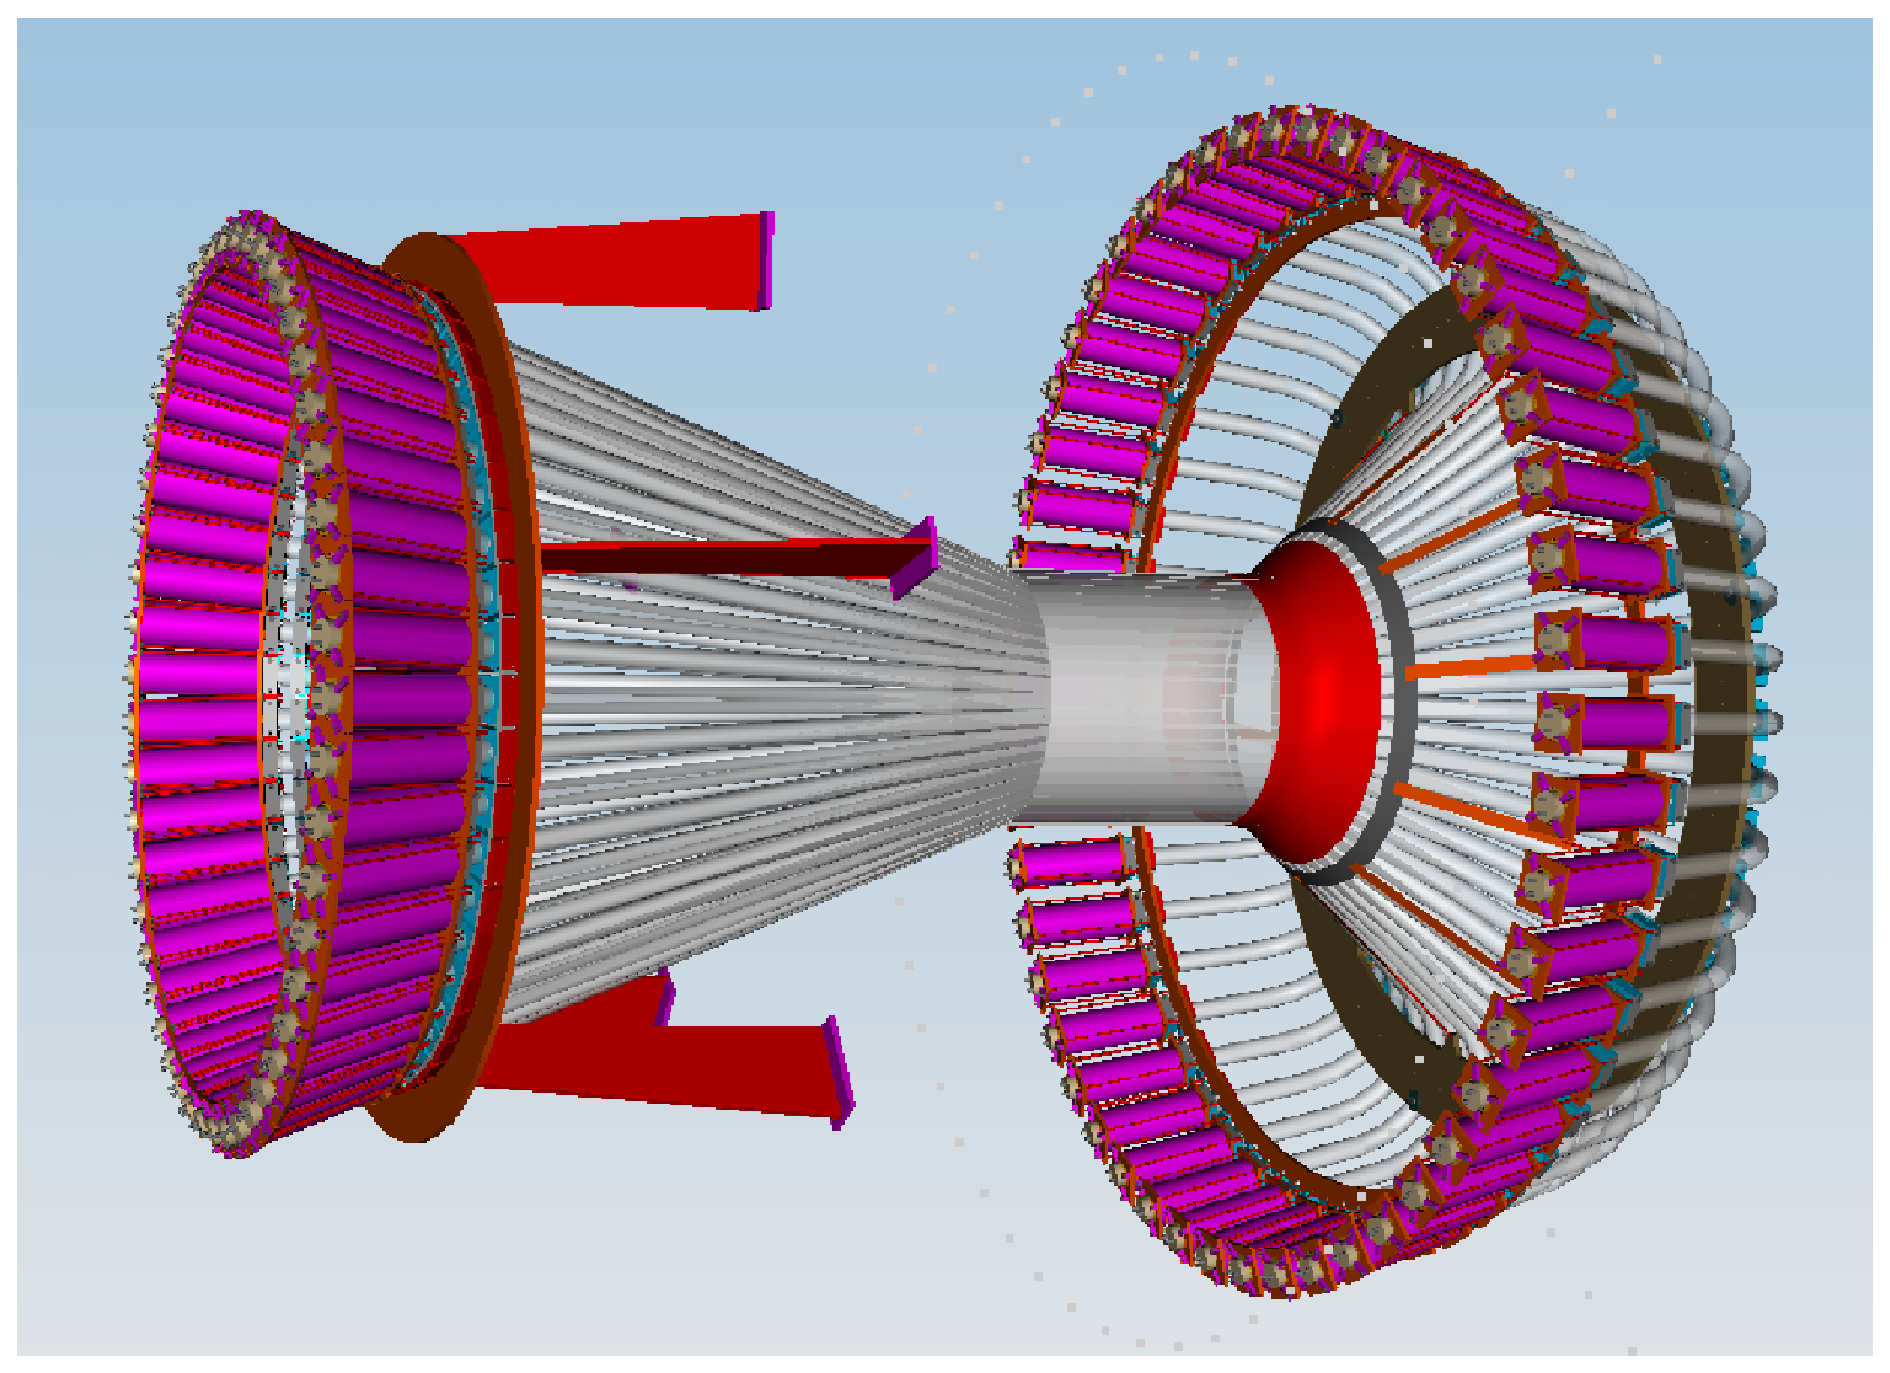
\includegraphics[height=4.90cm]{CTOFGELLYFISH1.eps}
\label{barrel1}}
\caption{(a). Cut view of the CLAS12 central solenoid and the layout of a portion 
of the CTOF detector. Only the upper half of the solenoid is shown. The beam is 
incident from the left. Labels: A - downstream PMTs, B - upstream PMTs, 1, $\cdots$, 
4 - PMTs of the High Threshold Cerenkov Counter (HTCC). (b). The 3D model of the 
CLAS12 CTOF detector.}
\label{fig:ctoffish}
\end{figure}
%%%%%%%%%%%%%%%%%%%%%%%%%%%%%%%%%%%%%%%%%%%%%%%%%%%%%%%%%%%%%%%%%%%%%%%%%%%%%%

With a triplet of identical prototyping CTOF counters, we have achieved a counter 
timing resolution of 55-60~ps in the Earth's magnetic field, using a double-sided 
readout~\cite{r1}-\cite{6percent}. However, the Hamamatsu R2083 PMT (our baseline
design choice) cannot retain its timing properties at inner fields higher than 0.5~G. 

The nominal central field of the CLAS12 solenoid is 5~T, therefore very long, straight 
or bent light guides are used to deliver the scintillation light to an area outside 
of the solenoid, where the associated high gradient fields are $\le$1000~G. Thus, our 
second goal is to design a magnetic shield that can preserve the timing properties of 
our readout PMTs and that allows us to minimize the length of the light guides.
   
In this paper we describe the development and test results of a robust magnetic shield 
for the CTOF PMTs. We strive for the extermination of the 1~kG external axial field to 
a level $\le$0.2~G inside the PMT, which may be considered a safe environment for 
optimal timing performance. With this goal in mind, we discuss the shield constraints 
and the design principles in Sections~\ref{sec:constr} and \ref{sec:principles}. In 
Section~\ref{sec:ednmics}, we describe a simplified theory of a ferromagnetic cylinder 
in an axial magnetic field. With this simple theory we have established an effective 
method  for the shield design and optimization using finite element analysis (FEA) 
calculations. In Section~\ref{sec:fea} we present our FEA simulations of various 
shielding designs and their optimization using the POISSON program~\cite{poisson}. 
With these tools, we have verified our design principles and designed the desired 
magnetic shields described in Section~\ref{sec:novelle}. In this section we also 
present our design for a novel dynamical magnetic shield for our PMTs. In 
Section~\ref{sec:tests} we report on our shield prototype tests, in particular on the 
shield effectiveness measurements in an external axial field of 1000~G. The prospects 
of using our shield design in the CLAS12 CTOF detector are discussed in 
Section~\ref{sec:concl}.   

\section{Design Constraints and Shield Dimensions}
\label{sec:constr}

In the current design of the CTOF, shown in Fig.~\ref{barrel1}, both the downstream 
and upstream PMTs are arranged in a circular pattern. The angle of the straight 
upstream light guides is dictated by minimum clearance dimensions with respect to the 
central tracking system. The downstream light guides are designed to extend around the
face of the solenoid while remaining outside of the HTCC volume. The light guide
length is set by reaching an external field of $\le$1000~G. However, the overall
length of the light guides needs to be minimized to optimize the timing resolution.
The system design and available space constrains the external dimensions of the
magnetic shield design.

Below we discuss issues of the shield design related to the shield diameter, the
external magnetic field, and the inner magnetic field at the location of the PMT.

\paragraph{Shield Diameter.}
The radial coordinates of the 50 adjacent shields on each end of the CTOF are 
constrained, therefore the spacing between the shields is limited. For the upstream 
side this limitation is more restrictive, however, a staggered design of the upstream 
light guides and PMTs allows for a common shield diameter constraint on both the
upstream and downstream ends of the CTOF. The design constrains the shield diameter
to be $\leq14.6$~cm.

\paragraph{External Field.}
The magnetic field map of the solenoid (Fig.~\ref{fig:mmap}) was studied and the 
appropriate PMT locations were determined via reckoning to provide a maximum  
magnetic field of 1000~G inside the area to be occupied by the magnetic shield. 
Following this restriction, the length of the upstream and downstream light guides
was determined to be 1.2~m and 1.5~m, respectively. At these positions relative to
the CLAS12 solenoid, the corresponding minimum magnetic fields in the shield area 
were in the range of 400-500~G. Thus, due to the high field gradient, the magnetic 
field drops by a factor of two across the shield dimensions. The shield orientation 
relative to the field direction is very important. Axial fields are the most 
difficult to eliminate. The calculated field pitch angles with respect to the PMT 
axis were $\approx15^\circ$ and $\approx45^\circ$ for the downstream and upstream PMTs, 
respectively. However, for a reasonable safety factor, we require the shields to 
operate in an external axial field up to 1000~G.

%%%%%%%%%%%%%%%%%%%%%%%%%%%%%%%%%%%%%%%%%%%%%%%%%%%%%%%%%%%%%%%%%%%%%%%%%%%%%%
\begin{figure}[htbp]
\centering
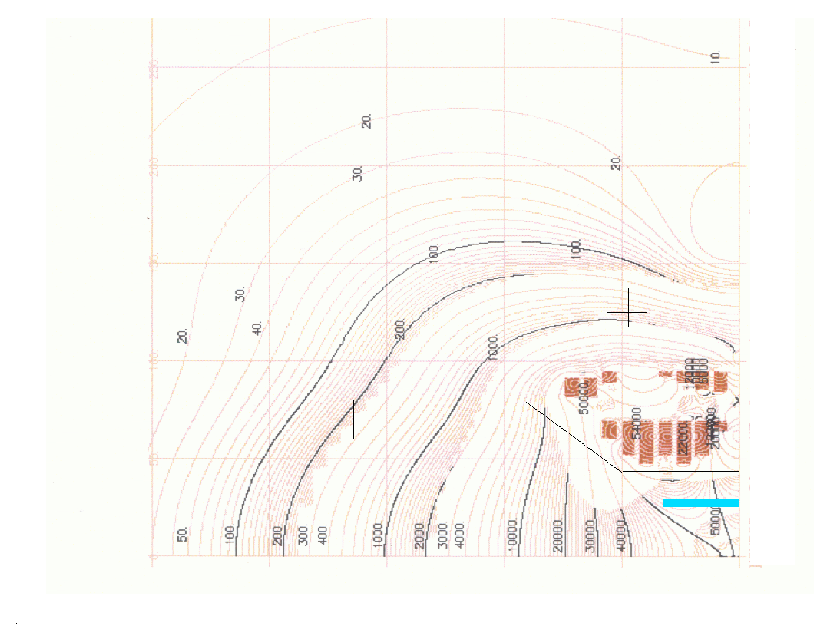
\includegraphics[height=6cm, clip=true,bb= 0 0 900 580]{mmap1.eps.gz}
%\includegraphics[height=6cm,clip=true,bb= 0 0 900 580]{SOLEN-B-MAP+PMTS.eps}
\caption{A quadrant of the axial symmetric field map of the CLAS12 central 
solenoid. The locations of both the upstream and downstream PMTs are shown with 
black rectangles. The bar in the bottom-right corner shows one half of the CTOF 
scintillator barrel cross section. The bent arrows indicate axial lines of 
corresponding light guides.}
\label{fig:mmap}
\end{figure}
%%%%%%%%%%%%%%%%%%%%%%%%%%%%%%%%%%%%%%%%%%%%%%%%%%%%%%%%%%%%%%%%%%%%%%%%%%%%%%

\paragraph{PMT Inner Field.}
The nominal readout choice for the CTOF is the Hamamatsu R2083 PMT. The diameter 
of its photocathode is 46~mm. As with most timing PMTs, it has a spherical 
photocathode. Such a shape is helpful to equalize travel distances of the primary 
photoelectrons. However, due to this spherical shape the accelerating electrical 
field always has a component perpendicular to an axial magnetic field. Therefore, 
timing PMTs are sensitive to the axial components of the magnetic fringe fields.

By design, the 46~mm diameter R2083 PMT is similar to the 76~mm diameter Photonis
XP4312 timing PMT, which is more sensitive to magnetic fields due to its larger 
diameter. The XP4312 PMT was thoroughly studied as a candidate for the CLAS TOF 
detectors~\cite{r2}. It was shown that an additional (in quadrature) time smearing 
of 20~ps appears due to residual fields of 0.4~G inside the PMT volume~\cite{flint}. 
We have also tested our reference phototube for its timing resolution in residual 
axial fields. Its timing performance was found to be stable even at 0.2-0.6~G in 
the most sensitive area between the first dynode and the photocathode.

Taking into account that the R2083 PMT is similar in design to the XP4312 PMT,
we allow for 0.4~G as the maximum allowable axial field at the photocathode.
However, we have aimed to achieve fields of $\leq$0.2~G to maintain a reasonable 
margin of safety.

\section{Principles of Shield Performance and Design}
\label{sec:principles}
 
The timing performance of photomultiplier tubes in external magnetic fields 
deteriorates due to the Lorentz force. After an external photon hits the surface 
of the photocathode and knocks out a primary electron, the electron accelerates 
towards the first dynode along the electric field lines. In most timing PMTs, the 
photocathode is shaped as a segment of a sphere. The first dynode is located close 
to the center of this sphere where the electric field lines concentrate. This
design provides about equal travel times for the electrons traveling from different 
parts of the photocathode. However, even an axial magnetic field has a transverse 
component to the electric field, and complex Lorentz forces affect both the 
propagation time and the destination of the electrons, depending on the design of 
the accelerating electrode. In designing magnetic shields for our PMTs, we have
been careful to consider both axial and transverse magnetic field components.

A PMT shield may be either active or passive. Active shielding makes use of
a compensating magnetic field produced by a solenoid around the PMT to cancel the 
internal field. We do not plan to use a traditional active shield for several 
reasons. First, in our case, the fringe fields are not solenoidal. Also, such a
shield would be complex and could be a source of additional electronic noise pickup.

The diamagnetic properties of a superconducting cylinder could be used for 
passive shielding. However, such a shield design is very complex and expensive, 
since it requires cryogenic cooling equipment.

Initially we consider a traditional passive shielding approach based on the 
properties of ferromagnetic cylinders. In such a passive shield, the magnetic 
field lines are concentrated in the bulk of the ferromagnetic material, reducing 
the fringing fields inside the cylinder. However, its effectiveness in high magnetic 
fields is limited by the maximum possible magnetization of the ferromagnetic 
material. This is a so-called saturating field, which is the most critical parameter 
affecting shield performance. 

In general, ferromagnets are available in two types, those with high saturation and 
those with high permeability. In very  high fields, cylinders  with high saturation 
should be used since a low saturation material would need to be excessively thick. 
Silicon steel (2.25\% Si, 0.40\% Al, balance Fe) (also known as electrical steel) may 
be used as a magnetic shield. It has been widely used in industry for relays and motors. 
It is easy to form and has a moderately high saturation field of 1.56~T, or up to
1.96~T if the grain pattern is oriented. The more advanced and expensive NETIC S3-6 
alloy from Magnetic Shield Corporation saturates at 2.14~T.

In moderate fields another high permeability material for shielding cylinders is 
Hiperm-49 (48\% Ni, 0.5\% Mg, 0.35\% Si, 0.02\% C, balance Fe). This may be used for 
an intermediate layer. This alloy has a saturation flux density of approximately 
1.5~T after hydrogen annealing.

Thin cylinders made of high permeability materials are useful in small magnetic fields. 
Therefore, they have been used as the innermost layer adjacent to the PMTs. One such 
material is CO-NETIC, an alloy that contains 80.6\% Ni and 14\% Fe, and is in the same 
family metallurgically as Mu-metal. It saturates at about 0.8~T.

Using coaxial cylinders meets the design  requirement that the magnetic shields must 
have openings for the coaxial light guides. Therefore, axial field lines can easy 
penetrate inside the shield. In order to eliminate this effect, we have developed a 
novel approach using a combination of passive and active elements. In this design, the 
compensating solenoid that makes up the active element controls the magnetization of 
the ferromagnetic layers, including the innermost layer, which determines the field 
within the PMT.

\subsection{Transverse Magnetic Fields}

The problem of an infinite hollow ferromagnetic cylinder in a uniform transverse 
magnetic field has been solved analytically~\cite{eltongluex}. The following
estimates are available for the magnetic shield parameters,

\begin{equation}
S=\frac{B_o}{B_{in}}\approx \mu({B_m})\frac{t}{D_+},~~~~~
B_m\approx B_o\frac{D_+}{0.8t},
\label{eq000}
\end{equation}

\noindent
where $S$ is the shielding factor, $B_o$ is the external field, $B_{in}$ is 
the field inside the shielding cylinder, $\mu(B_m)$ is the permeability as a 
function of the field $B_m$ inside the ferromagnetic material, $D_+$ ($D$) is 
the outer (inner) diameter of the shield cylinder, and $t$ is the shielding 
material thickness. 

For a multi-layer shield of $n$ coaxial cylinders separated by $\approx 1$~mm in 
radius, the resulting shielding factor may be estimated as

\begin{equation}
S=S_1 \times S_2 \times...\times S_n,
\label{eq777}
\end{equation}

\noindent
where $S_i,i=1,...,n$ is the shielding factor for the $i^{th}$ cylinder, estimated 
via Eq.~\ref{eq000}. Due to this relation, multi-layer shields are typically more 
effective than a single-layer shield of the same net material thickness.

%%%%%%%%%%%%%%%%%%%%%%%%%%%%%%%%%%%%%%%%%%%%%%%%%%%%%%%%%%%%%%%%%%%%%%%%%%%
\begin{table}[htbp]
\begin{center}
\begin{tabular}{|c|c|c|c|c|c|c|c|c|} \hline
Cyl &$B_{o}$ & $D_+$ & $t$ & $B_m$ & $\approx\mu$ & $S$ & $B_{in}$ & $Fm$ \\
$n$ &  G     & mm    & mm  & G     &             &     & G       &   \\ \hline
1   & 1000& 86 & 9.94 & 10800 & 5000   & 872  & 1.2   & NETIC \\ \hline
2   & 1.2 & 64 & 0.8  &  120  & 100000 & 1250 & 0.001 & CO-NETIC \\ \hline
\end{tabular}
\end{center}
\caption{R2083 PMT shielding in a transverse 1000-G field. ($n$)~-~layer 
number starting from the external layer, ($B_{o}$)~-~external field,
($D_+$)~-~outer shield diameter, ($t$)~-~ferromagnetic thickness, ($B_m$)~-~
bulk ferromagnetic field, ($\mu$)~-~permeability, ($S$)~-~shielding factor,
($B_{in}$)~-~shielding inner field, ($Fm$)~-~ferromagnetic material.}
\label{ca001}
\end{table}
%%%%%%%%%%%%%%%%%%%%%%%%%%%%%%%%%%%%%%%%%%%%%%%%%%%%%%%%%%%%%%%%%%%%%%%%%%%

An example of shield performance evaluation using Eq.~\ref{eq777} is given
in Table~\ref{ca001}. Since Eq.~\ref{eq000} was obtained for a two-dimensional 
shield, i.e. for an infinitely long cylinder, the shield length is not a parameter 
of the problem. According to this table, the task of reducing a transverse 1000-G 
field to a level below 0.1~G inside a 20-cm-long PMT may be easily solved with two 
layers of coaxial ferromagnetic cylinders with a total weight of only a few kg.
 
The effectiveness of a two-layer shield was confirmed by two-dimensional FEA
calculations in a transverse field (see Fig.~\ref{shieldGrilli}). These 
calculations were performed for a slightly different shield configuration where 
the outer layer is a 2.54-cm-thick, 250-mm-long soft iron cylinder with an external 
diameter of 136~mm. The inner layer is a 1.6-mm-thick Hiperm-49 cylinder, 84~mm in 
outer diameter. The minimum field inside this shield is about 0.23~G in a 3000~G 
external transverse magnetic field. Hence, we conclude that transverse 1000-G 
fields may be easily exterminated at the PMT with a shield consisting of 2 to 3 
layers of ferromagnetic coaxial cylinders.  
 
In practice all cylinders are of a finite length. However, as is well known from 
experimental measurements, at a distance of one shield diameter inside the ends 
of the shield, the inner fields along the shield axis are as for an infinite cylinder. 
Therefore, common sense requires that each subsequent external layer be 
correspondingly longer and longer. However, as will be shown in the next section, 
this design solution may not work in axial fields.

%%%%%%%%%%%%%%%%%%%%%%%%%%%%%%%%%%%%%%%%%%%%%%%%%%%%%%%%%%%%%%%%%%%%%%%%%%%
\begin{figure}[htbp]
%\vspace{7.5cm}
%\special{psfile=magshieldGrilli-1.ps.gz hscale=55 vscale=55 hoffset=80 voffset=-5}
%\special{psfile= Grilli-copy.eps hscale=1 vscale=1 hoffset=-100 voffset=100}
\centering
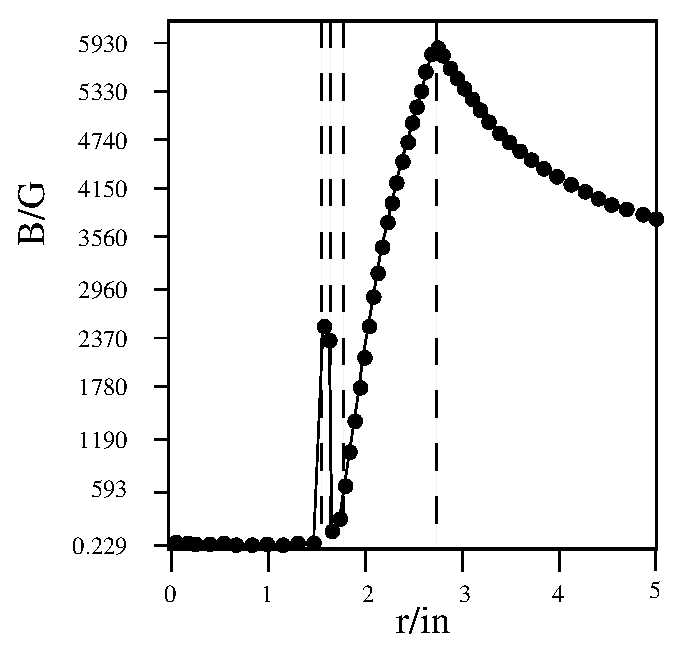
\includegraphics[height=6cm]{Grilli-copy.eps}
\caption{FEA calculation of the magnetic flux density $B$ inside two coaxial 
cylinders at a transverse field of 3000~G~\cite{grilli}. Vertical scale - B/G. 
Horizontal scale - radial distance r/in. The vertical dashes lines indicate the
inner and outer diameters of the two shield cylinders.}
\label{shieldGrilli}
\end{figure}
%%%%%%%%%%%%%%%%%%%%%%%%%%%%%%%%%%%%%%%%%%%%%%%%%%%%%%%%%%%%%%%%%%%%%%%%%%%

In Section~\ref{sec:ednmics} we consider the electrodynamics of ferromagnetic 
cylinders in an axial field. From simple analytical estimates we learn that 
shielding dynamics are very different from the transverse field case, and that 
the longitudinal dimensions of the shield cylinders are of crucial importance to 
optimize the shielding factor $S$. 

\subsection{Axial Magnetic Fields}
\label{sec:ednmics}

Finite element analysis of shield models is the most appropriate method for 
shield development and our FEA studies~\cite{dynshi,wieland} are reported in 
Section~\ref{sec:fea}. However, an unambiguous interpretation of FEA results
for complex shields is impossible without a clear understanding of the 
electrodynamics of ferromagnetic cylinders in axial fields.

The magnetization of a ferromagnetic may be modeled assuming that its inner space 
is filled with randomly oriented magnetic dipoles, or current loops. Dipoles of a 
certain density are responsible for local magnetization under an external field, 
which aligns the dipoles along the field direction. As a result, the inner 
ferromagnetic fields are amplified by orders of magnitude. However, outside the 
ferromagnet the resulting field drops, since in that region the common field of 
current loops is in the direction opposite to the original field. This is the basic 
mechanism of magnetic shielding.

Effectively, only a surface current protects the inner space of a shielding 
cylinder, since the internal currents cancel each other in the bulk of the 
ferromagnetic material. Due to the cylindrical symmetry, the surface currents run 
in the azimuthal ($\phi$) direction. Here, due to the circular pattern of the inner 
currents, the current over the inner surface of a cylinder will be in the opposite 
direction to that on the outer surface. Therefore, a ferromagnetic cylinder can be 
approximated by two thin coaxial solenoids with opposite currents (see 
Fig.~\ref{flatcylinder}). The inner solenoid has a diameter $D$, while the outer 
solenoid has a diameter $D+2t$, where $t$ is the thickness of the cylinder.

%%%%%%%%%%%%%%%%%%%%%%%%%%%%%%%%%%%%%%%%%%%%%%%%%%%%%%%%%%%%%%%%%%%%%%%%%%%
\begin{figure}[htbp]
\centering
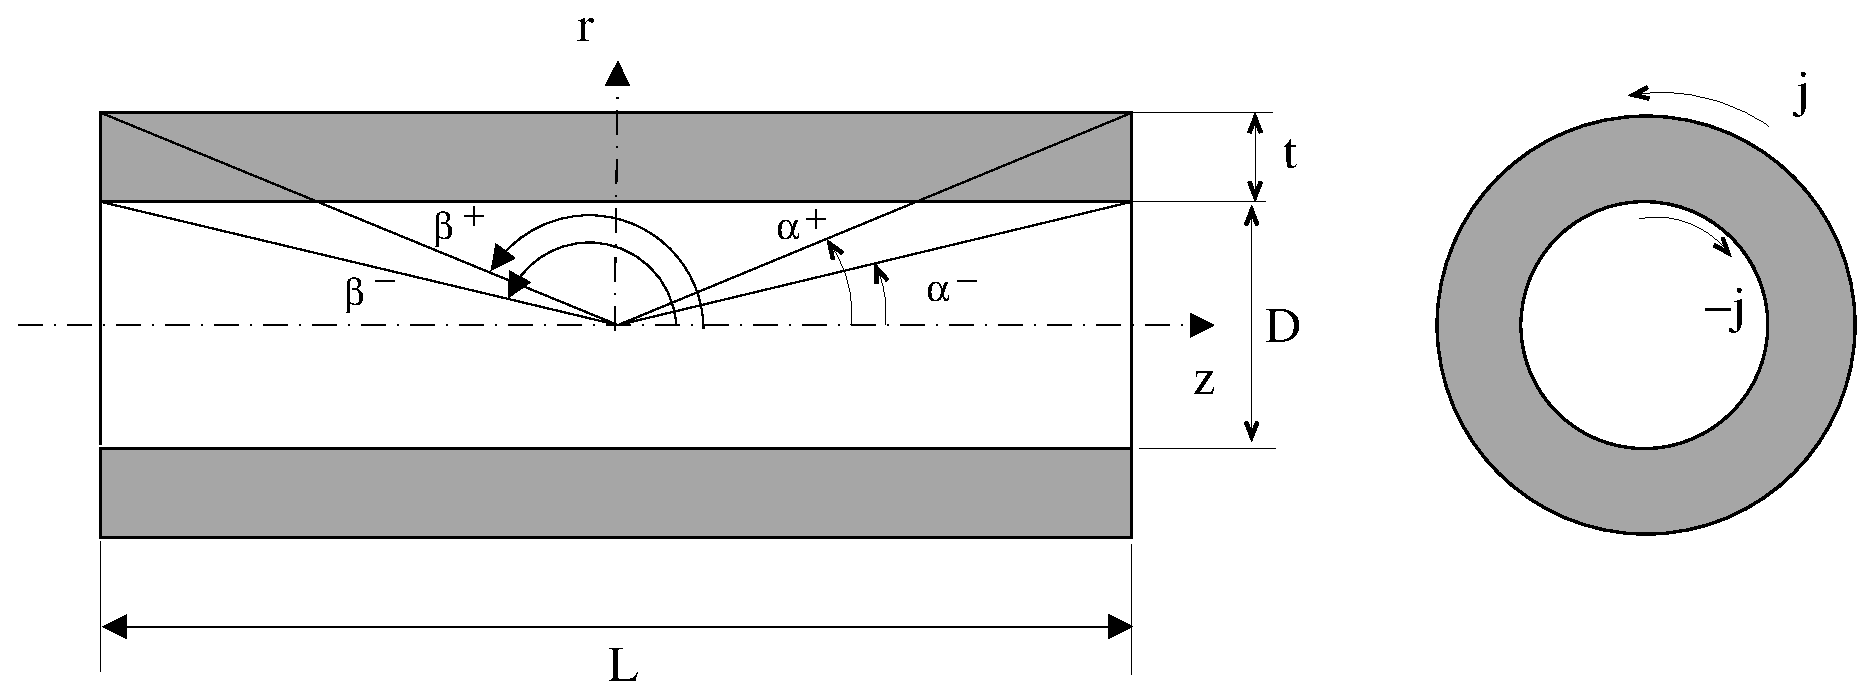
\includegraphics[width=12cm]{flatcylinder.eps}
\caption{Approximation of a ferromagnetic cylinder in an axial magnetic field
by two infinitely thin cylinders with opposite surface currents $j$. The cylinder 
length is $L$, inner diameter $D$, and thickness $t$. The four angles involved 
from Eqs.~\ref{eq:eq31} and \ref{eq:eq32} are shown for the $z=0$ case.}
\label{flatcylinder}
\end{figure}
%%%%%%%%%%%%%%%%%%%%%%%%%%%%%%%%%%%%%%%%%%%%%%%%%%%%%%%%%%%%%%%%%%%%%%%%%%%

Using a known formula for a finite solenoid~\cite{jackson}, we can evaluate the 
magnetic field $B_+(z)$ induced by the external magnetic field on the outer surface 
of our ferromagnetic shield cylinder: 

\begin{equation}
B_+(z)=+\frac{1}{2}\mu_0 j_s \left( \cos \alpha^+(z) - \cos \beta^+(z) \right),
\label{eq:eq31}
\end{equation}

\noindent
where $\mu_0$ is the permeability of free space, $j_s$ is the absolute value of the 
surface current density per unit length, and $\alpha^+(z)$ and $\beta^+(z)$ are 
the angles between the $z$-axis and the two vectors between the point $z$ and the 
corresponding ends of the cylinder (see Fig.~\ref{flatcylinder}). Due to the opposite 
direction of the inner surface currents, the corresponding field $B_-(z)$ can be
written as

\begin{equation}
B_-(z)=-\frac{1}{2}\mu_0 j_s \left(\cos \alpha^-(z) - \cos \beta^-(z) \right),
\label{eq:eq32}
\end{equation}

\noindent
where the angles $\alpha^-(z)$ and $\beta^-(z)$ are defined in Fig.~\ref{flatcylinder}.
Thus, the resulting field inside the shield, $B_{in}$, may be evaluated from 
the following relation:

\begin{eqnarray}
B_{in}\!\!\!\!&-&\!\!\!\!B_o = B_+ - B_- = \\ \nonumber
&-&\!\!\!\!\!\mu_0 j_s
\left[ \sin \left(\frac{\alpha^+ + \alpha^-}{2} \right) \sin\left(\frac{\alpha^+ - 
\alpha^-}{2}\right) - \sin \left( \frac{\beta^+ + \beta^-}{2}\right)
\sin \left(\frac{\beta^+ - \beta^-}{2}\right) \right].
\label{eq:eq1}
\end{eqnarray}

\noindent
From this equation we make the following surprising observation: as the shield
length increases, $B_{in}$ tends to the external field value $B_o$, since all   
terms containing angles in this equation tend to zero. In other words, unlike in 
the transverse field case, an excessively long shield does not work for the case
of an axial magnetic field. 

Let us now estimate the field in the center of a ferromagnetic cylinder, i.e. at 
$z=0$ for a purely axial external field. For the trigonometric functions in 
Eqs.~\ref{eq:eq31} and \ref{eq:eq32} in the center of the cylinder we write:

\begin{equation}
\cos\alpha^+(0)=-\cos\beta^+(0)=\frac{1}{\sqrt{1+\left(\frac{D+2t}{L}\right)^2}}~, \nonumber
\label{eqcos1}
\end{equation}
\begin{equation}
\cos\alpha^-(0)=-\cos\beta^-(0)=\frac{1}{\sqrt{1+\left(\frac{D}{L}\right)^2}}~.
\label{eqcos}
\end{equation}

\noindent
Using Eqs.~\ref{eqcos} for direct evaluation of $B_+(0)$ and $B_-(0)$ via 
Eqs.~\ref{eq:eq31} and \ref{eq:eq32}, respectively, and assuming that $t \ll D$ 
we find:

\begin{equation}
B_{in}(0) - B_o = B_+(0) - B_-(0) \approx - \mu_0 j_s  \frac{t}{D} \frac{2x^2} 
{(1+x^2)^{\frac{3}{2}}} = -\mu_0 j_s \frac{t}{D} g(x),
\label{eq101}
\end{equation}

\noindent
where we define $g(x)$ as a function of $x=D/L$. The inner field $B_{in}(0)$ in 
Eq.~\ref{eq101} is connected to the ferromagnetic properties of the shield 
material via the surface current density $j_s$. With this relation, we note that 
in the Maxwell equation

\begin{equation}
\vec{\nabla} \times \vec{H} = \vec{j},
\label{eqHJ}
\end{equation}

\noindent
the current density $\vec{j}$ is the sum of the external current density
$\vec{j}_e$ and the surface current density $\vec{j}_s$. Integrating 
Eq.~\ref{eqHJ} over a rectangular loop enclosing the inner surface element in 
the middle of the solenoid\footnote{Here the radial components may be neglected.}, 
we find for the magnetic intensity $\vec{H}$,

\begin{equation}
H_m^z =H_{in}^z+j_s,
\label{eqBJ1}
\end{equation}

\noindent
where $H_m^z$ is the $z$-component in the bulk of the ferromagnetic material, 
$H_{in}^z$ is the field along the axis, and $j_s$ is the $\phi$ component of 
the surface current density that scales in units of current per unit length. 
Thus, multiplying Eq.~\ref{eqBJ1} by $\mu_0$, we obtain the relation

\begin{equation}
B_m = B_{in}(0) + \mu_0 j_s = \mu(B_m)B_{in}(0),  
\label{eqBJ}
\end{equation}

\noindent
where, by definition, $\mu(B_m)$ is the $B_m$-dependent permeability of the  
ferromagnetic material. Using Eq.~\ref{eqBJ} to exclude the term $\mu_0 j_s$ 
from Eq.~\ref{eq101}, we find:

\begin{equation}
B_{in}(0) = B_o - (\mu(B_m) - 1) \frac{g(x)t}{D} B_{in}(0).
\label{eq11}
\end{equation}

\noindent
Thus, using Eq.~\ref{eqBJ} to exclude $B_{in}(0)$ from Eq.~\ref{eq11}, we find 
the relation between the magnetization $B_m$ of the ferromagnetic material and 
the external field $B_o$,

\begin{equation}
B_o = \left( (\mu(B_m)-1)\frac{g(x)t}{D}+1 \right) B_{in}(0) 
\approx \frac{g(x)t}{D}B_{m},
\label{eq12}
\end{equation}

\noindent
where we have used the fact that in most practical cases, $\mu(B_m)\gg1$. Finally, 
from Eq.~\ref{eq12}, we determine the magnetization of the ferromagnetic material
as

\begin{equation}
B_{m} = B_o\frac{D}{g(x)t}.
\label{eq121}
\end{equation}

\noindent
Substituting Eq.~\ref{eq11} into Eq.~\ref{eq12} and using Eq.~\ref{eq121} as an 
argument for $\mu(B_m)$, we find the final relation between the external and 
internal fields as

\begin{equation}
B_o \approx \mu\bigg(B_o 
\frac{D}{g(x)t}\bigg) \frac{g(x)t }{D} B_{in}(0) = S \times B_{in}(0),
\label{eqfinal}
\end{equation}

\noindent
where $S$ defines the shielding factor. Note that $g(x)$ defined in Eq.~\ref{eq101}
tends to zero for long and short cylinder lengths, and has a maximum at 
$x=\sqrt2$. Therefore, for constant or slowly varying permeability, one may  
expect the maximum of shield effectiveness (or maximum $S$) to occur at 
$D \approx \sqrt{2}L$. We verify this prediction using FEA in Section~\ref{sec:fea}.

An important practical rule may be  concluded from Eq.~\ref{eqBJ}. Assume  
that a tiny piece of ferromagnetic, a probe, is in close contact with the 
inner surface of our ferromagnetic cylinder. The external field induces 
surface currents in both materials. For the case of close contact, the surface 
currents must be identical, otherwise this would violate the law of charge  
conservation. Therefore, the magnetization of the probe must be equal 
to that of the ferromagnetic layer. Thus, we conclude that in order to 
provide independent performance of different coaxial layers, contact between  
the ferromagnetic layers must be avoided.

\section{Finite Element Analysis of Coaxial Cylinders}
\label{sec:fea}

In this section we describe our FEA studies of coaxial ferromagnetic cylinders
in an external axial magnetic field. Our goal is to develop a robust magnetic 
shield for our linear-focused PMT. We also verify the predictions of our 
simplified theory, which were found to be very successful in interpretations of 
often surprising FEA results.

The magnetic field has been calculated using the POISSON program~\cite{poisson}. 
This program performs two-dimensional net calculations in axial $z$-symmetric 
fiducial spaces of limited sizes. The magnetic field in this space has been 
created by an infinitely thin solenoid, the size of which is significantly larger 
than all of the shield dimensions. The field magnitude has been controlled by
varying the current running through the solenoid. The magnetic shield has been 
placed inside the solenoid. The boundary conditions, required by the POISSON 
program, were selected to enforce that the field lines be parallel to the 
fiducial space borders. Thus, one may consider both the shield and the 
solenoid as confined inside a large diamagnetic box.

\subsection{Single-Layer Ferromagnetic Shield}
\label{emsdimen}

In this section we consider an example of POISSON calculations for a 
single-layer magnetic shield constructed from a 6-mm-thick iron cylinder. Such 
a shield may house the Hamamatsu metal-channel H8500 PMT. It has been considered 
as an alternative for the Hamamatsu R2083 PMT in the CTOF detector due to its 
ability to operate in axial magnetic fields up to 100-200~G without significant 
loss of timing resolution. Therefore, for external axial fields as high as 
1000-2000~G, the shielding factor may be as low as 10. 

The field map produced by POISSON is shown in Fig.~\ref{Upstream_PMT_Design} 
together with the shield design. Shown in this figure is actually one quadrant 
of the full axis-symmetric configuration with the bottom-left corner being the 
center of the shield. The shield is a flanged iron cylinder, 0.6-cm thick, about 
14-cm long with an inner diameter of 7.62~cm. A quarter of the PMT, such as the 
Hamamatsu metal-channel H8500, may occupy a box with $(z,r)$ (cm) coordinates 
(0,0) and (1,3) with the photocathode located at $z$=1~cm. The opening at
$z$$\approx$7~cm is for the 2-in diameter light guide that delivers light to the 
photocathode.

%%%%%%%%%%%%%%%%%%%%%%%%%%%%%%%%%%%%%%%%%%%%%%%%%%%%%%%%%%%%%%%%%%%%%%%%%%%
\begin{figure}[htbp]
\centering
\subfloat[]
{\includegraphics[height=4cm,clip=true,bb=00 00 790 590 ]{H8500_Upstream_NETIC_6mmThick_69mmLength.eps}
\label{Upstream_PMT_Design}}
\qquad
\subfloat[]
{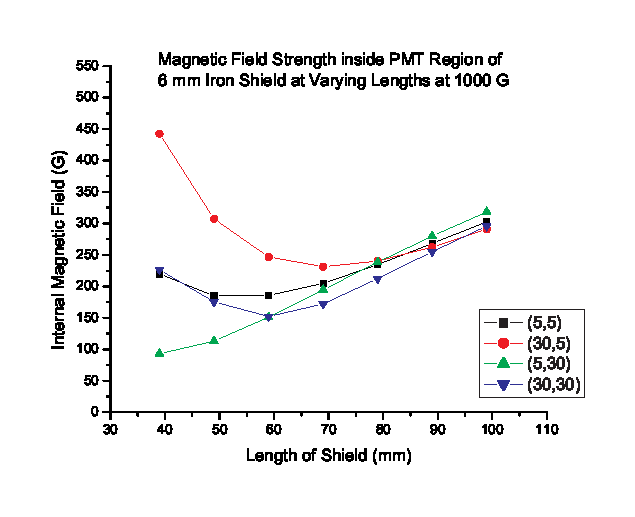
\includegraphics[height=4cm,clip=true,bb= 15 15 290 180]{H8500_Upstream_SingleIron_6mm_Thick_PMT_Region.eps}
\label{fig:BIN8500}}
\caption{(a). One quadrant of the POISSON model for a single-layer ferromagnetic 
shield (6-mm-thick iron) and the calculated field map for a 1000~G external axial 
magnetic field. Horizontal scale - $z$/mm; vertical scale - $r$/mm. The PMT model  
occupies a box with $(z,r)$-coordinates (0,0) and (30,30). (b). Magnetic field in 
the PMT region as a function of one half of the model shield length. The magnetic 
field values were measured at four reference points with coordinates labeled as 
$(z,r)$.}
\label{fig:SH8500}
\end{figure}
%%%%%%%%%%%%%%%%%%%%%%%%%%%%%%%%%%%%%%%%%%%%%%%%%%%%%%%%%%%%%%%%%%%%%%%%%%%

This shield is not a  perfect cylinder. As can be seen from 
Fig.~\ref{Upstream_PMT_Design}, the narrowing on the ends helps to capture more
field lines at low radial coordinates compared to a flat cylinder. This feature 
results in a lower inner field with better uniformity along the central axis.

Due to the high permeability of the shield material, the field lines refract at the 
boundary to be almost parallel to the ferromagnetic surface. Therefore, a shield 
without an aperture at the ends would be more effective to reduce the inner field 
level. However, this is not possible due to the requirement of having an opening 
for the cylindrical light guide.

Using POISSON model calculations, we have verified the simple theory developed in 
Section~\ref{sec:ednmics}. That was a tremendous step to understanding the 
shield performance. The shielding factor $S$ determined in Eq.~\ref{eqfinal} is 
given as

\begin{equation}
S=\mu\bigg(B_o \frac{D}{g(x)t}\bigg) \frac{t }{D} \frac{2x^2}{(1+x^2)^{\frac{3}{2}}},
\label{eqfinal1}
\end{equation}

\noindent
where $x=D/L$. A surprising prediction from this expression is that $S$ is maximal 
at $D =\sqrt{2}L$ and tends to zero at low and  high values of $L$ for a fixed 
shield diameter $D$. 

When we allow the length to increase, the external cylinder captures more and more 
field lines. Therefore, at a certain length we expect a complete ``collapse'' of 
the shield performance to occur. The key point is that due to the high permeability 
of the shield material, the vacuum field lines are about normal to the ferromagnetic 
surface, while inside the ferromagnetic material, they run about parallel to it. 
Hence, the magnetization in the median plane ($z=0$) of the ferromagnetic will climb 
with increasing length of the cylinder. At a certain value of $L$, the ferromagnetic 
saturates and additional normal field lines penetrate into the center of the cylinder. 
We refer to this surprise as a ``dimensional effect'', which has been confirmed in our 
POISSON calculations as well.

The calculated field inside the shield as a function of the shield length is shown in
Fig.~\ref{fig:BIN8500}. The following reference points are addressed in this figure. 
Two points with coordinates at $z$=5~mm are close to the median plane where the first 
dynode of the PMT will be located. Two additional reference points are placed at 
$z=30$~mm, i.e. close to the location of the PMT photocathode. It is seen from 
Fig.~\ref{fig:BIN8500}, that there is a pronounced minimum at a shield length 
of 50-60~mm, which agrees\footnote{The shield length in the POISSON model is one half 
of the full length.} with the prediction of Eq.~\ref{eqfinal1}. This observation allows 
us to optimize the overall shield length.

A magnetic shield with optimized length was tested for two thicknesses. The same 
four reference points are addressed in both cases. In 
Fig.~\ref{Upstream_Iron_4mm_PMT_Region} the four reference points inside the 
4-mm-thick iron shield are examined at varying external axial fields. The curves 
in Fig.~\ref{Upstream_Iron_21mm_PMT_Region} for a 21-mm-thick iron shield show that 
this design is sufficient for the Hamamatsu metal-channel H8500 PMT up 1250-2000~G. 
It is important to understand that the metal-channel dynodes occupy the space at 
$z$$\approx$5~mm where, according to this figure\footnote{Curves labeled as (5,5) 
and (5,30).}, the field magnitude remains below 100-200~G up to 1250-2000~G of 
external field. Using the higher saturation NETIC ferromagnetic for the shield
material provided 20\% better performance over the use of iron in terms of the
maximum tolerable axial field.

However, neither of these shields is capable of providing inner fields below 
a few Gauss. This is due to the axial structure of the problem, and requires an
improved multi-layer shield design to further reduce the inner magnetic field 
levels. 

%%%%%%%%%%%%%%%%%%%%%%%%%%%%%%%%%%%%%%%%%%%%%%%%%%%%%%%%%%%%%%%%%%%%%%%%%%%
\begin{figure}[ht]
\centering
\subfloat[]
{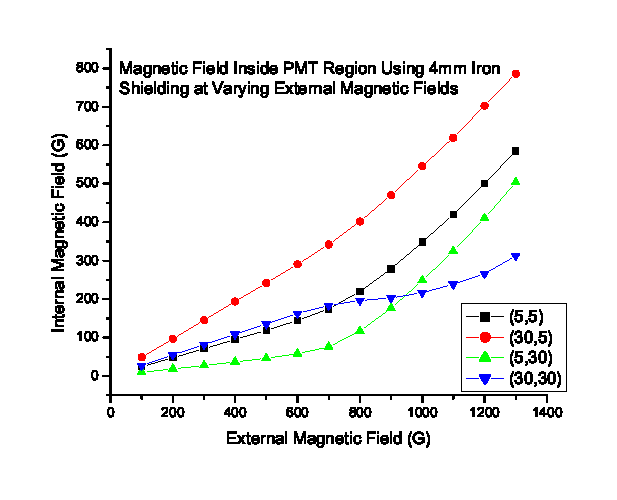
\includegraphics[height=5cm]{H8500_Upstream_SingleIron_4mm_Thick_PMT_Region.eps}
\label{Upstream_Iron_4mm_PMT_Region}}
\qquad
\subfloat[]
{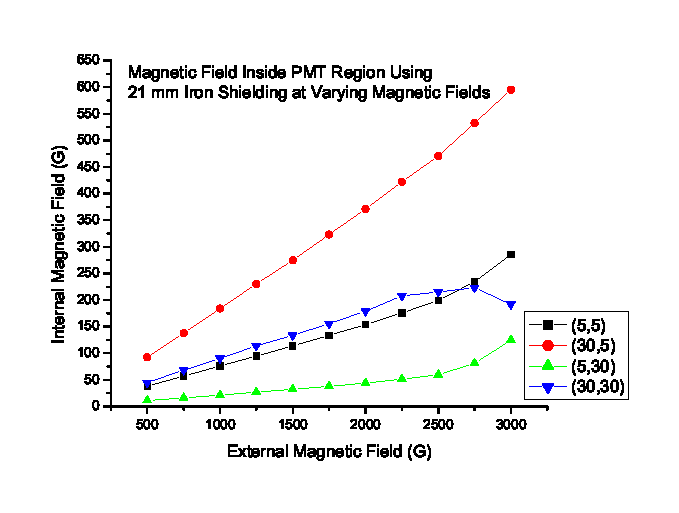
\includegraphics[height=5cm]{H8500_SingleIron_21mm_Thick_PMT_Region.eps}
\label{Upstream_Iron_21mm_PMT_Region}}
\caption{Magnetic field at four reference points within the PMT for varying external 
axial magnetic fields. (a). Inside a 4-mm-thick iron shield, (b). inside a 21-mm-thick 
iron shield. The coordinates of the reference points are labeled as $(z,r)$ (mm).}
\label{Upstream_Iron_4mm}
\end{figure}
%%%%%%%%%%%%%%%%%%%%%%%%%%%%%%%%%%%%%%%%%%%%%%%%%%%%%%%%%%%%%%%%%%%%%%%%%%%

\subsection{Triple-Layer Ferromagnetic Shield}
\label{sec:tlfs}

Axial field lines easy penetrate into the PMT region. In order to capture more of 
the axial lines, additional ferromagnetic material has to be included in the 
shield. The most straightforward solution would be to enclose the PMTs within a 
ferromagnetic ellipsoid. Unfortunately, this cannot work due to the opening 
required for the cylindrical light guides. An assembly of a cylinder with end caps 
may work as an approximation for the ellipsoid. Here, the end cap should have an 
axial hole for the light guide. 
 
To proceed, we consider a multi-layer shield design for the linear-focused 
photomultipliers. In this design each subsequent external layer should be longer 
than the previous layer to avoid the aforementioned dimensional effect (see 
Section~\ref{emsdimen}). A viable shield design and the corresponding POISSON field 
map for a 1000~G external axial magnetic field are shown in Fig.~\ref{SH2083}. The 
inner layer is of a fixed size and material - 0.8-mm-thick high permeability mu-metal, 
similar to CO-NETIC, which is a part of the Hamamatsu H2431 assembly with our main 
R2083 phototube inside. The outermost shield has a maximum thickness of 1.7~cm due to 
the CTOF design constraints. It may be either soft iron (low-carbon iron) or NETIC. 
The middle shielding layer is composed of 3~mm of Hiperm-49 with moderate permeability. 
However, within the shield design limitations, varying sizes for the middle layer of 
the shield were tested, as well as the utilization of both NETIC and iron in the 
outer layer. Similar to the design in Fig.~\ref{Upstream_PMT_Design}, the external 
cylinder has a flange that helps to capture field lines close to the axis. The middle 
layer is flanged with the same goal. The holes in the flanges are for the 2-in
diameter cylindrical light guide.
  
%%%%%%%%%%%%%%%%%%%%%%%%%%%%%%%%%%%%%%%%%%%%%%%%%%%%%%%%%%%%%%%%%%%%%%%%%%%
\begin{figure}[ht]
\centering
\subfloat[]
%{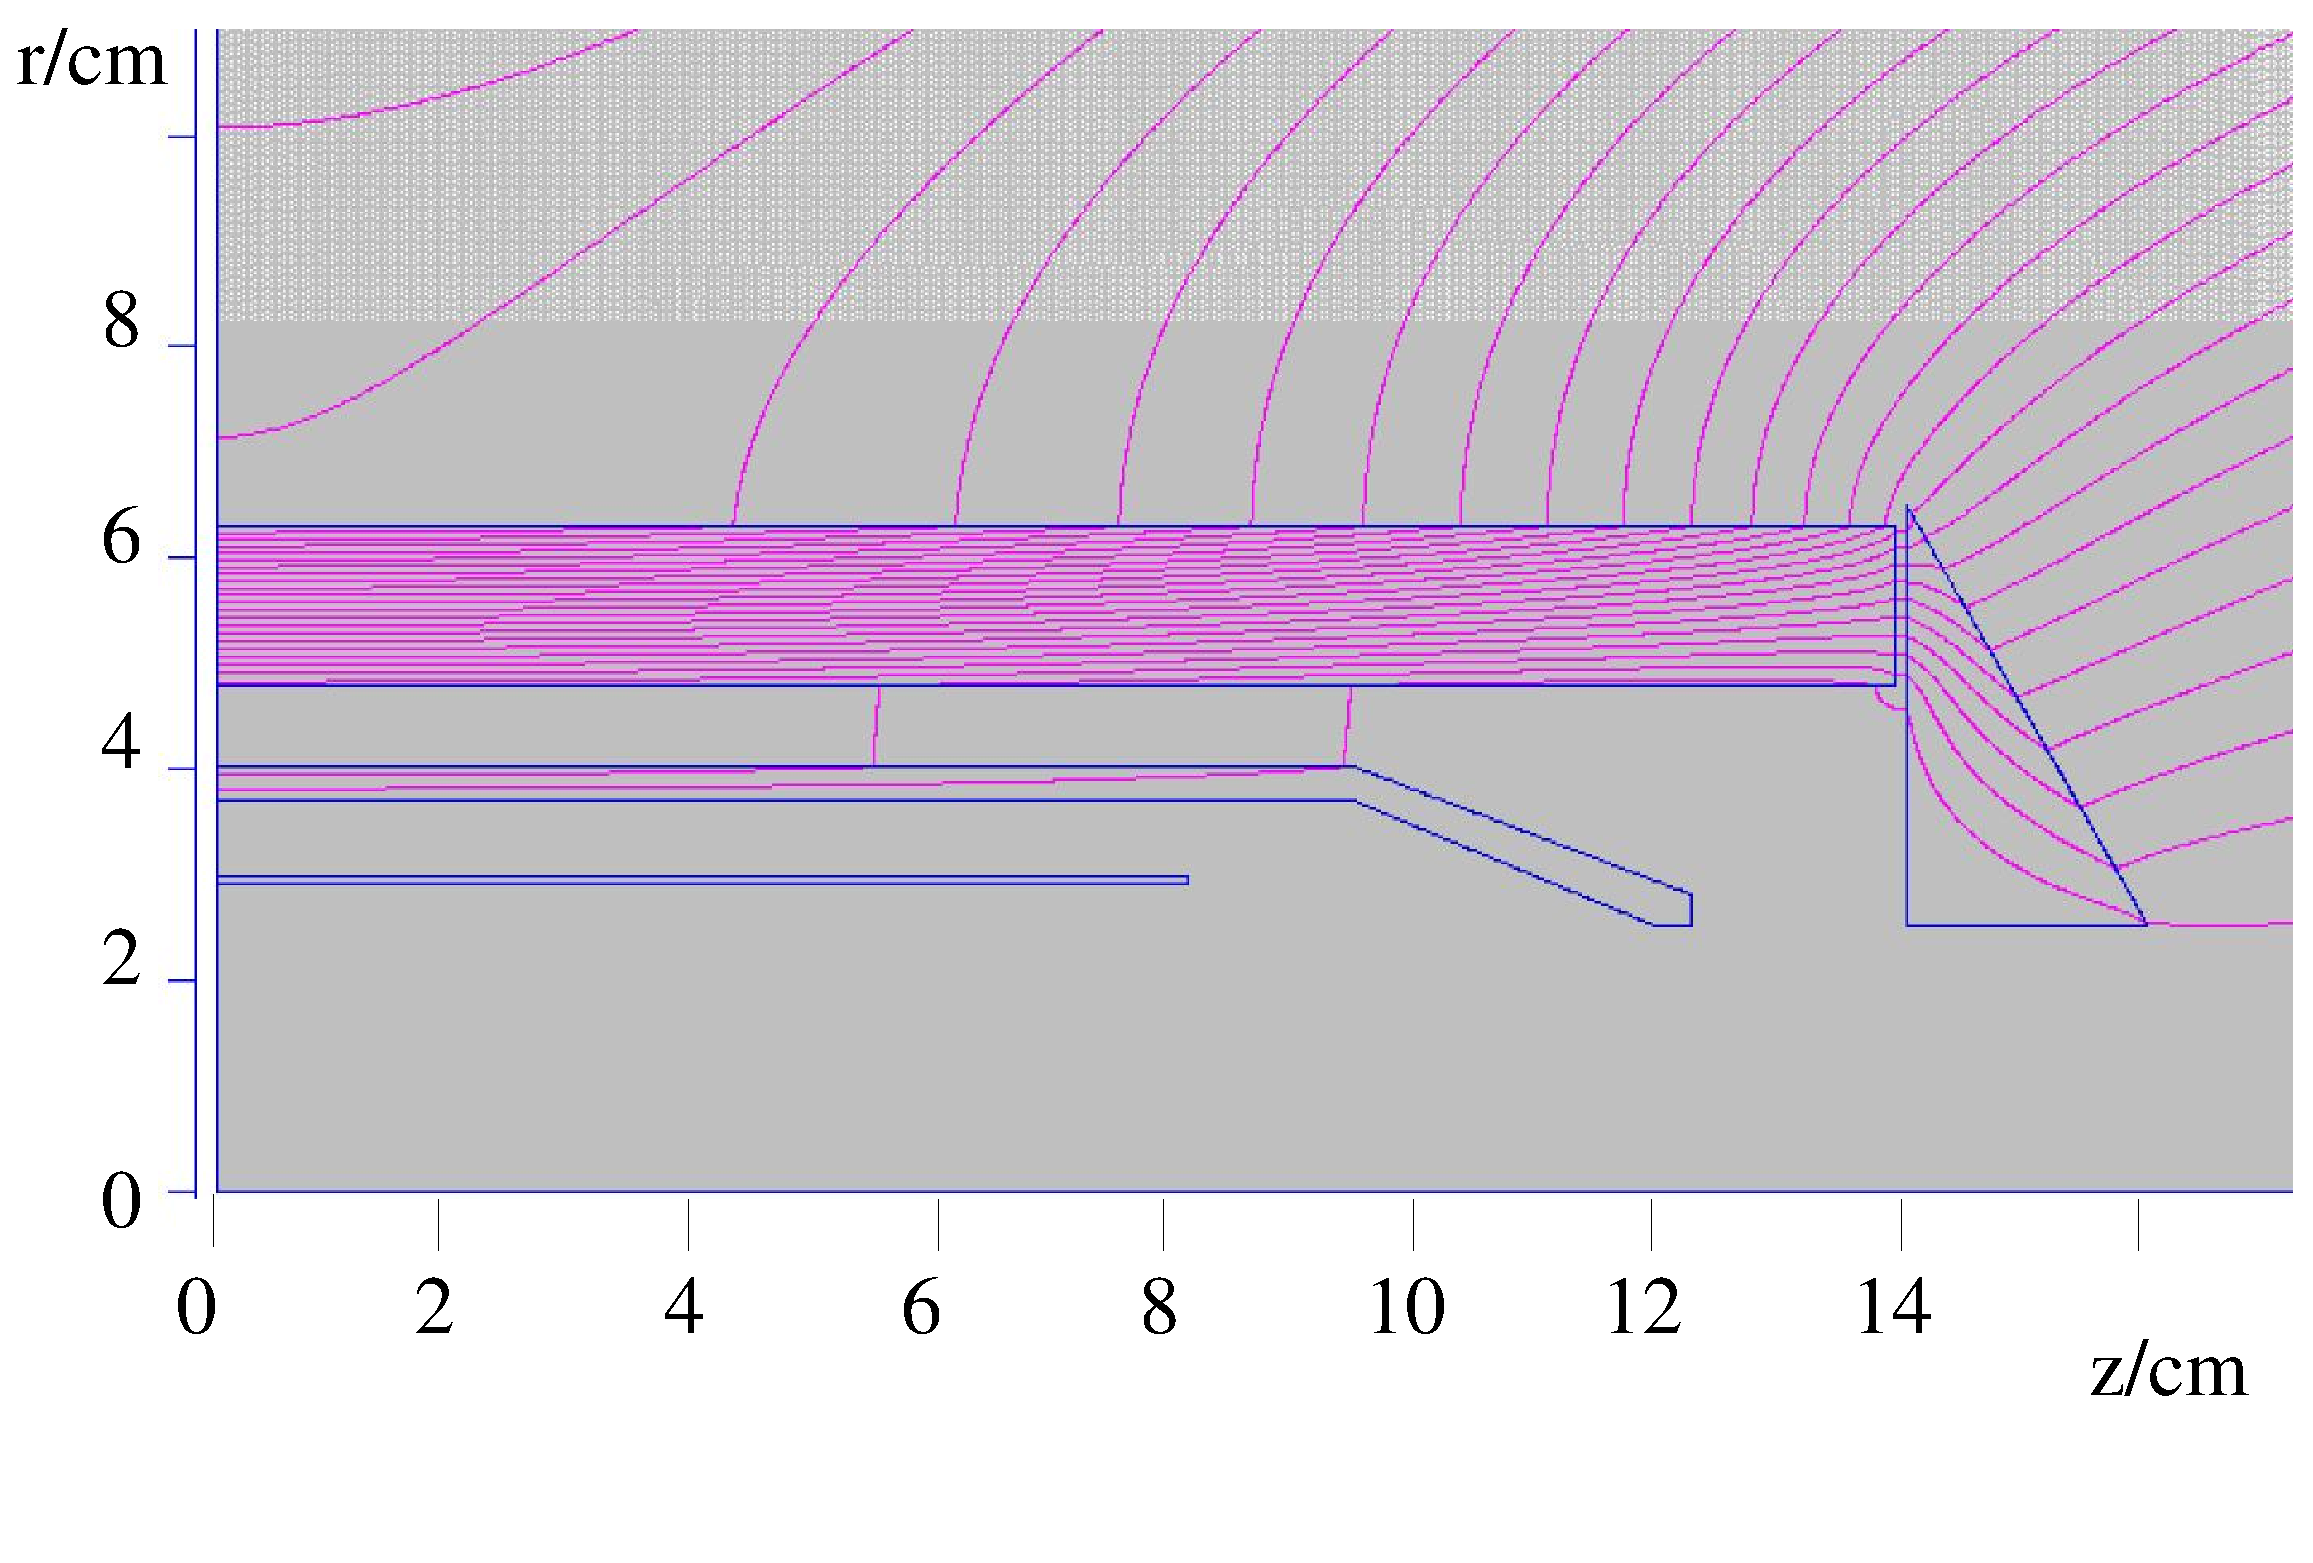
\includegraphics[height=4cm,clip=true,bb=10 -50 1350 600]{R2083_NETIC_hiperm49_CONETIC_standardDesign.eps}
{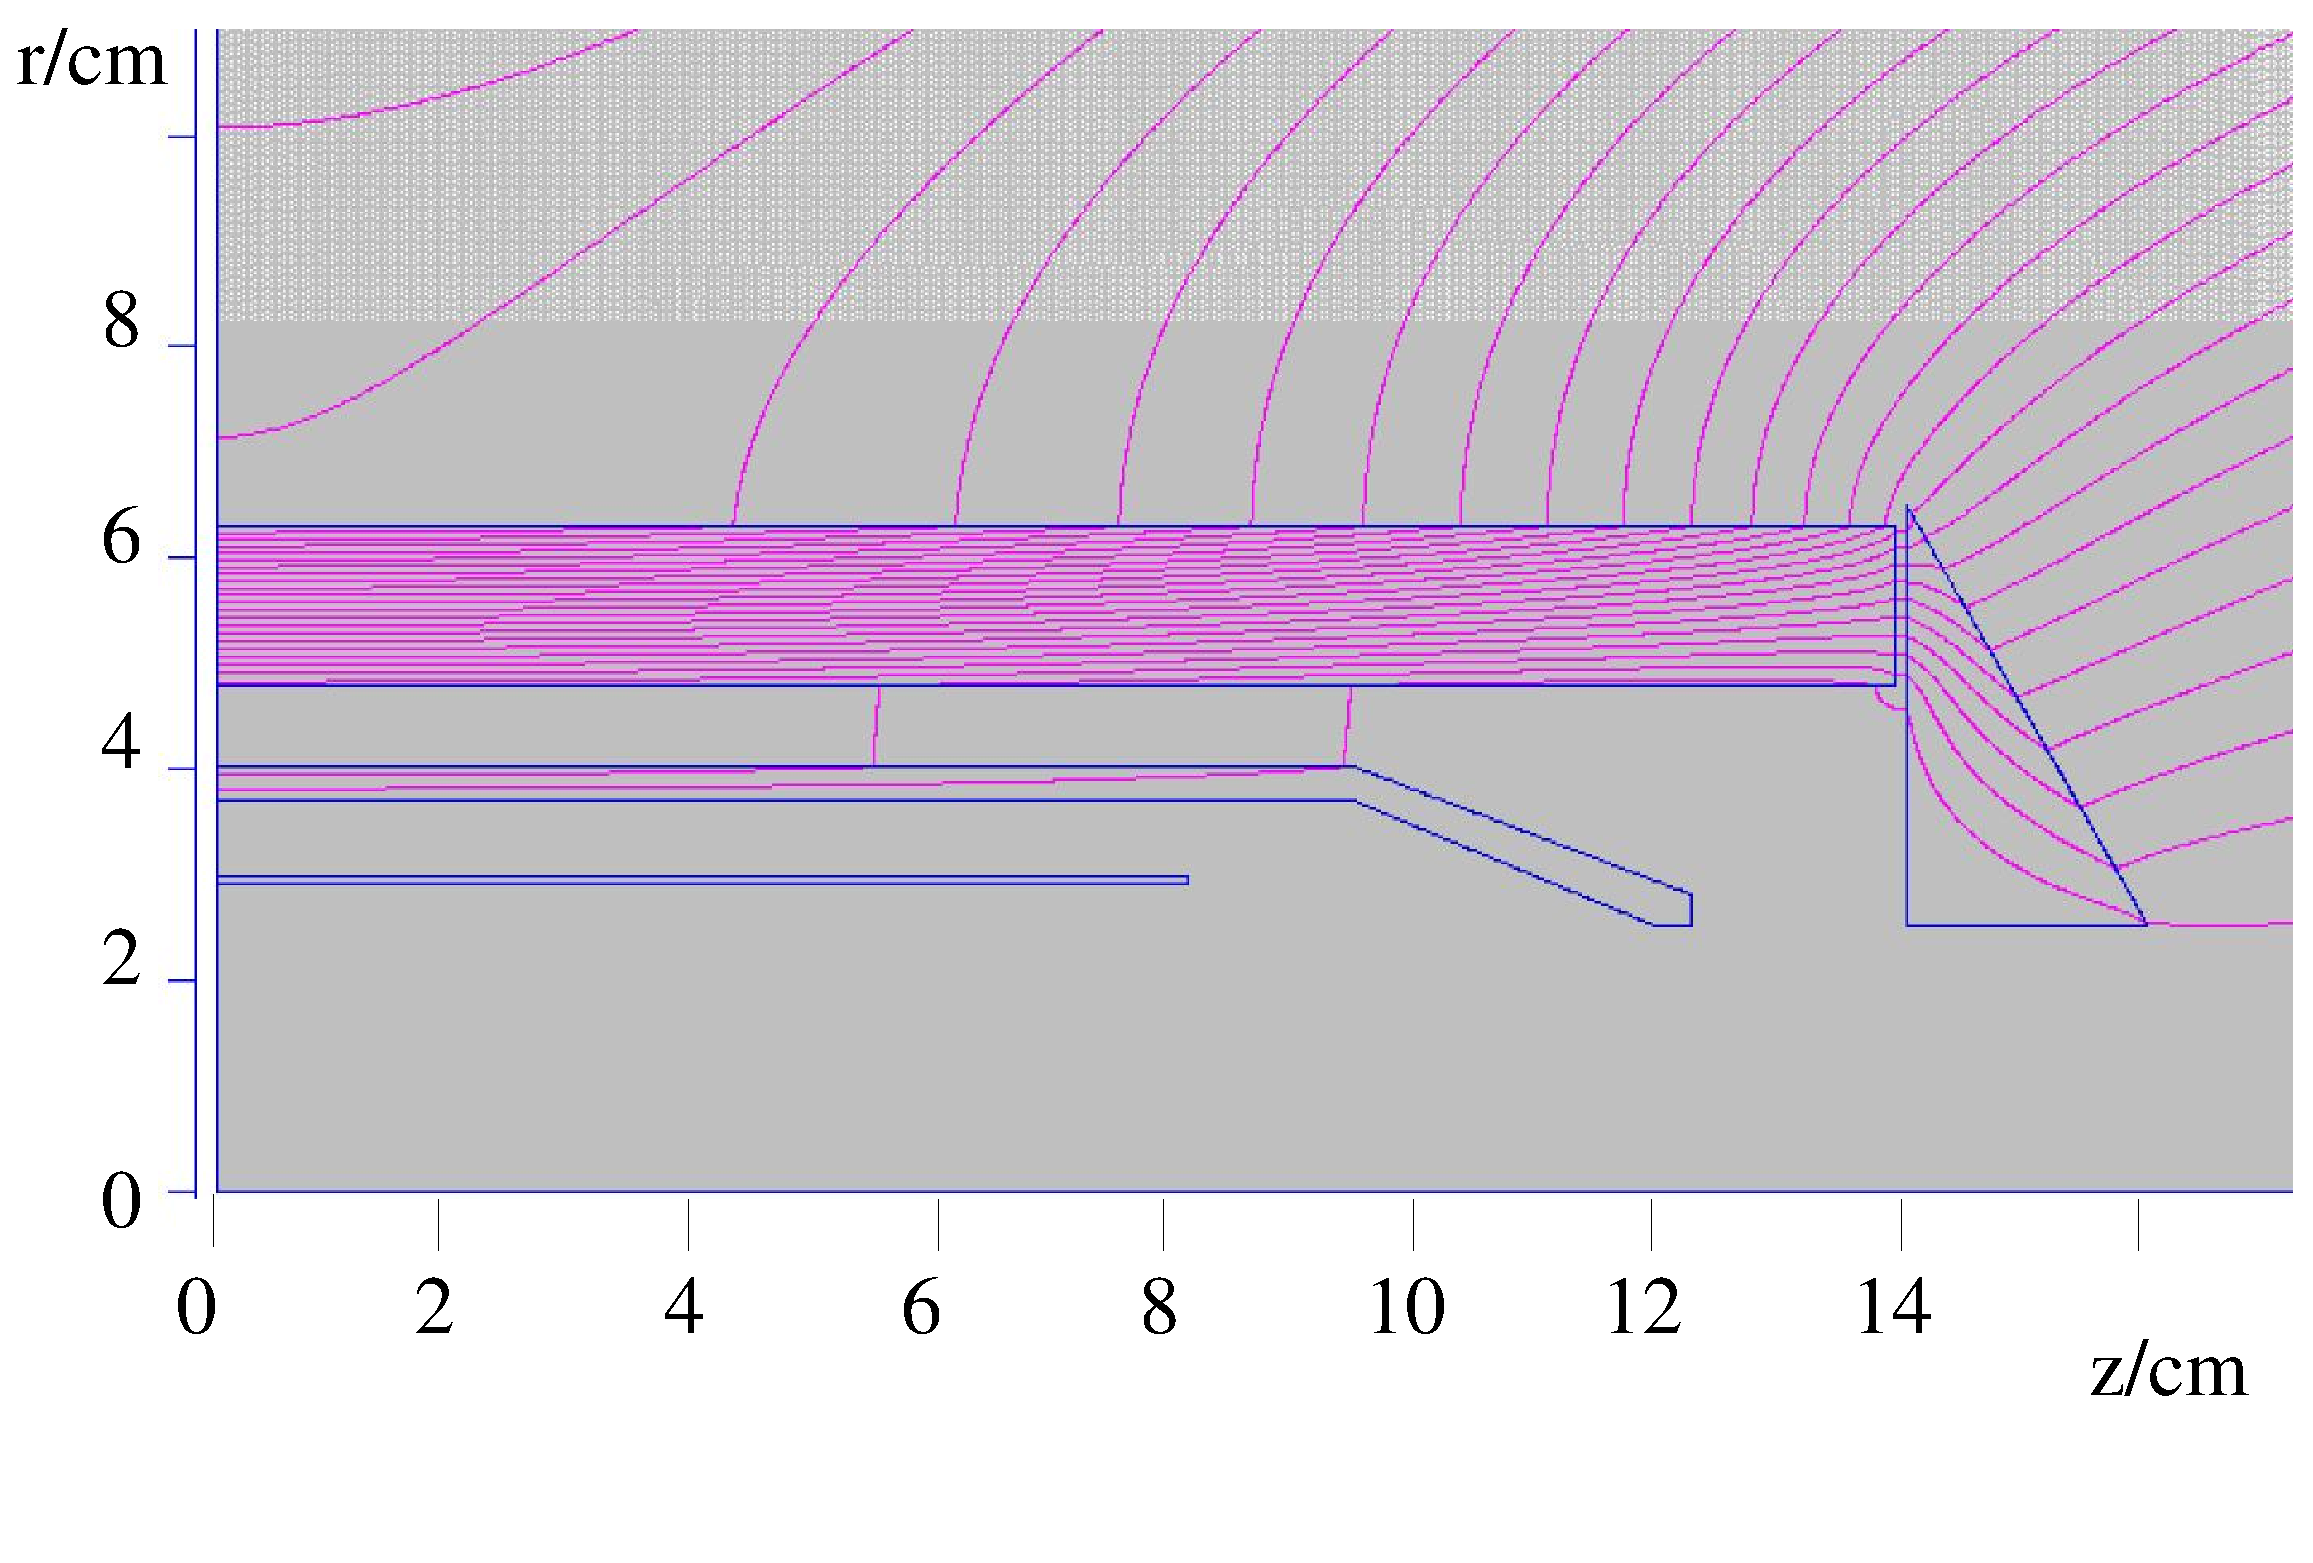
\includegraphics[height=4cm,clip=true,bb=0 60 1150 750]{R2083_NETIC_hiperm49_CONETIC_standardDesign.eps}
\label{SH2083}}
\qquad
\subfloat[]
{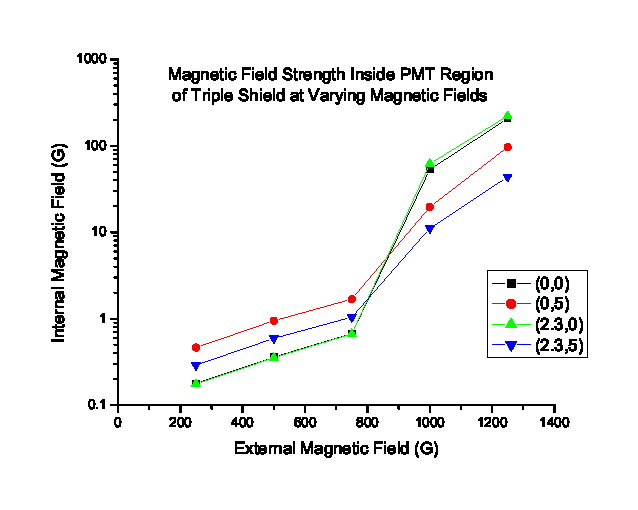
\includegraphics[height=4cm,clip=true,bb= 15 15 290 180]{R2083_Iron_hiperm49_CONETIC_0.3mm_PMT_Region.eps}
\label{BSH2083}}
\qquad
\caption{(a). One quadrant of the POISSON model for a triple-layer ferromagnetic shield 
in a 1000~G external axial magnetic field. Horizontal scale - $z$/cm; vertical scale - 
$r$/cm. In this plot the PMT occupies a box with $(z,r)$-coordinates (0,0) and (5,2.3)
(b). Magnetic fields at four reference points inside the PMT region labeled as 
$(r,z)$.}
\label{R2083_Initial_Iron}
\end{figure}
%%%%%%%%%%%%%%%%%%%%%%%%%%%%%%%%%%%%%%%%%%%%%%%%%%%%%%%%%%%%%%%%%%%%%%%%%%%

Although the PMT is not shown in Fig.~\ref{SH2083}, it occupies a box with 
$(z/{\rm cm},r/{\rm cm})$-coordinates of (0,0) and (5,2.3). The PMT photocathode 
is located at $z$=5~cm. We have assumed that remnant fields of up to 0.2~G within 
the inner shield are acceptable for the high resolution operation of our timing PMTs.

Shields with different materials were tested at varying external magnetic fields 
from 250~G to 1250~G. For each external field setting, we monitored four reference 
points\footnote{All points are given in $(r,z)$ form and are expressed in cm.}.
Two points are inside the sensitive region of the PMT with coordinates (0,0) and 
(2.3,0), where the first PMT dynode is situated. Our other two points are at the 
PMT photocathode with coordinates (0,5) and (2.3,5). In order to control saturation 
effects, we also monitor the fields in the bulk of the ferromagnetic layers.

The resulting field values for the reference points are shown in Fig.~\ref{BSH2083}.
At all reference points, the inner field increases slowly with increasing external 
field up to $\approx$750~G. After that the inner field values climb very rapidly. 
The behavior of the bulk ferromagnetic field indicates this effect is due to the 
saturation of the external layer. Therefore, we refer to this field value as the 
critical field. As seen from Fig.~\ref{BSH2083}, at the saturation point the central 
field is about 0.5~G, which exceeds our design limit of 0.2~G. Moreover, the field 
values increase towards the open ends of the shield due to the penetrating axial 
field lines. At the photocathode, the field value is higher than 1~G. Using NETIC 
for the external layer results in only a $\approx$20\% higher critical field. The 
inner fields still remain within the interval 0.5-1~G. To further reduce the inner 
field levels, we have increased the thickness of the middle layer from 3~mm to 8~mm. 
As a result, the critical field value increased by another 20\%.

Although these tests show quite good shield performance, the inner fields remain 
significantly higher than the tolerable limit of 0.2~G, even at an external field of 
250~G. Moreover, the outer shield layer has already reached its maximum thickness as 
allowed by the current CTOF design. Hence, we conclude that the three-layer 
ferromagnetic shield is not sufficient in the environment of the CTOF detector. 
Further increase of shield length is not possible due to the dimensional effect, 
while the transverse dimensions are constrained by the detector design. Thus a fully 
passive multi-layer ferromagnetic shield for the CTOF design is not possible given 
our constraints. In Section~\ref{sec:novelle} we describe a novel hybrid 
ferromagnetic shield that allows us to attain fields below 0.2~G in both the 
upstream and downstream CTOF PMTs in external axial fields of up to 1000~G.

\section{Novel Dynamical Magnetic Shields}
\label{sec:novelle}

As was shown in Section~\ref{sec:ednmics}, the inner field of a shielding 
cylinder is determined by the magnetization of the ferromagnetic material.
Here, the relation between the magnetization and the shield inner field is 
determined via the boundary conditions at the inner surface of the ferromagnetic 
cylinder (Eq.~\ref{eqBJ}). Our main idea is to control the magnetization of the 
innermost shield cylinder using a solenoid as an active shield layer. The 
solenoid is wound around a ferromagnetic component, i.e. it is placed outside the 
shielding cylinder, and its current is set to reduce the magnetization of the 
ferromagnetic material. Thus, the field inside the cylinder is also reduced due to
the aforementioned boundary conditions. 

We refer to this combination of passive and active shielding elements as 
a ``hybrid shield'' or ``dynamical magnetic  shield''(DMS). In Section~\ref{sec:tests} 
we show that with such a shield, it is possible to attain inner fields below 
0.2~G in external axial fields as high as 1000~G.

We emphasize that the demagnetizing  solenoid should be placed outside the 
ferromagnetic cylinder. The whole point is that the effective field in the PMT 
area is a superposition of the ferromagnetic magnetization, the residual external 
fields, and the solenoidal field. Consider a contrary situation, where the 
solenoid is placed inside the ferromagnetic cylinder. If we assume the solenoid 
field to be opposite to the residual external field, then the solenoidal external 
flux is collinear to the residual external field. Therefore the solenoid induced 
magnetization of the cylinder would add coherently with the external field. Thus, 
unlike the case of an external demagnetizing solenoid, the inner solenoid creates 
two opposite axial fields. The first field is the field of the demagnetizing 
solenoid, and the second field, with opposite direction, is due to the additional 
ferromagnetic magnetization by the solenoid external field. Numerous POISSON 
calculations have convinced us that the two opposing fields do not compromise in 
the PMT area, especially at high external fields. Typically the result was a high 
and non-uniform inner field with frequent ``collapse'' owing to a saturated 
ferromagnetic layer. 

\subsection{Upstream Dynamical Shields (Moderate Field)}

Our first three-layer ferromagnetic shield with a demagnetizing coil (DMS) is 
shown in Fig.~\ref{VBT3CYUS1}. The external iron cylinder is 7.62~cm in diameter, 
28-cm long, and 0.6-cm thick. The end cap includes an opening for the 2-in diameter 
light guide and is attached for better uniformity of the resulting inner field. The 
middle layer of shielding is made of 0.32-cm-thick Hiperm-49. 

A coil of 200 winds of 1-mm-thick wire is placed between the middle and the innermost 
layers. The current through the coil\footnote{The POISSON model specifies the current 
through the model half-plane in $A\times W$inds.} was set to about 0.5~A. In the 
POISSON coordinates, the coil winding spans from $z$=4~cm to 14~cm. The real coil would 
span from -14~cm to +14~cm with an 8-cm-gap in the middle. Such a gap helps to achieve 
a more uniform field along the PMT axis with a very low field magnitude in the area of 
the R2083 PMT photocathode. As seen from  Fig.~\ref{VBT3CYUS1}, the PMT occupies a box 
with $(z/{\rm cm},r/{\rm cm})$ limits of (0,0) and (5,2.3). A more detailed field map 
inside the PMT region at 400~G is shown in Fig.~\ref{VBT3CYUS2}. According to this 
figure, the demagnetizing coil allows the inner PMT field to be below 0.1~G. 
Moreover, the field magnitude is quite uniform over a wide area.

%%%%%%%%%%%%%%%%%%%%%%%%%%%%%%%%%%%%%%%%%%%%%%%%%%%%%%%%%%%%%%%%%%%%%%%%%%%
\begin{figure}[ht]
\centering
\subfloat[]
%{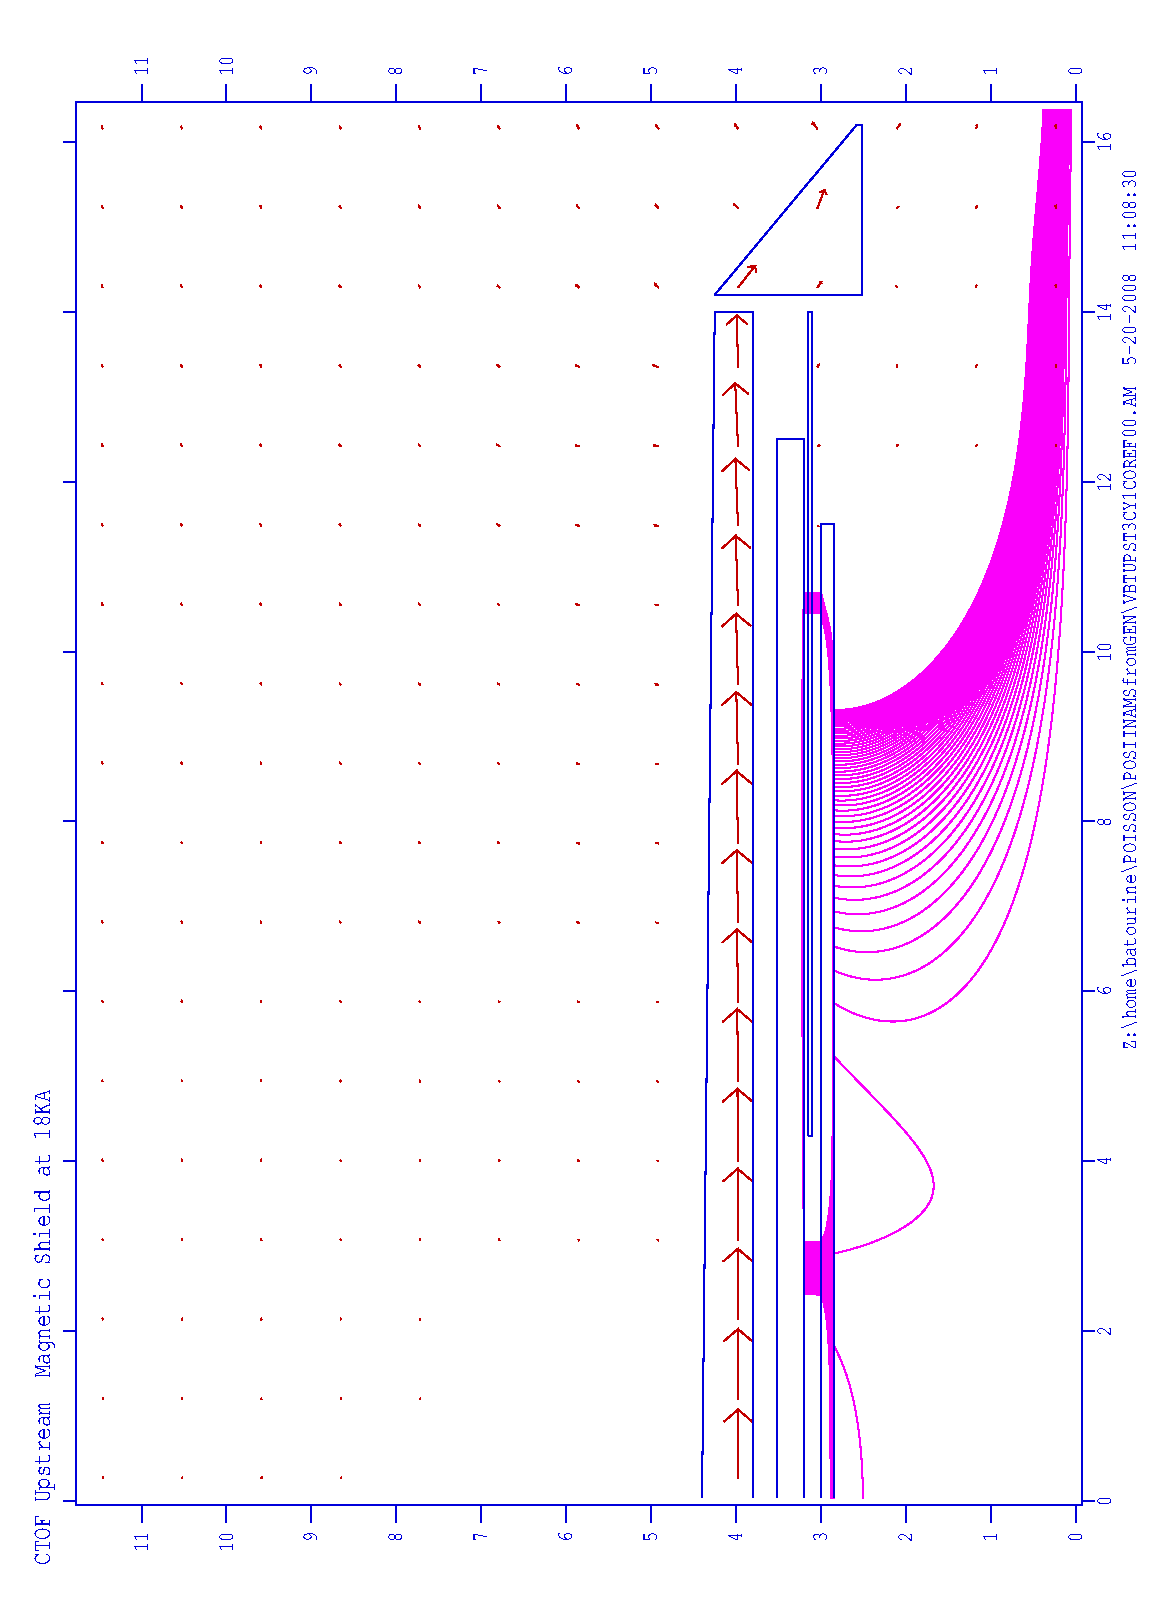
\includegraphics[height=7cm,angle=-90]{VBTUPST3CY1COREF0001.eps}\label{VBT3CYUS1}}
{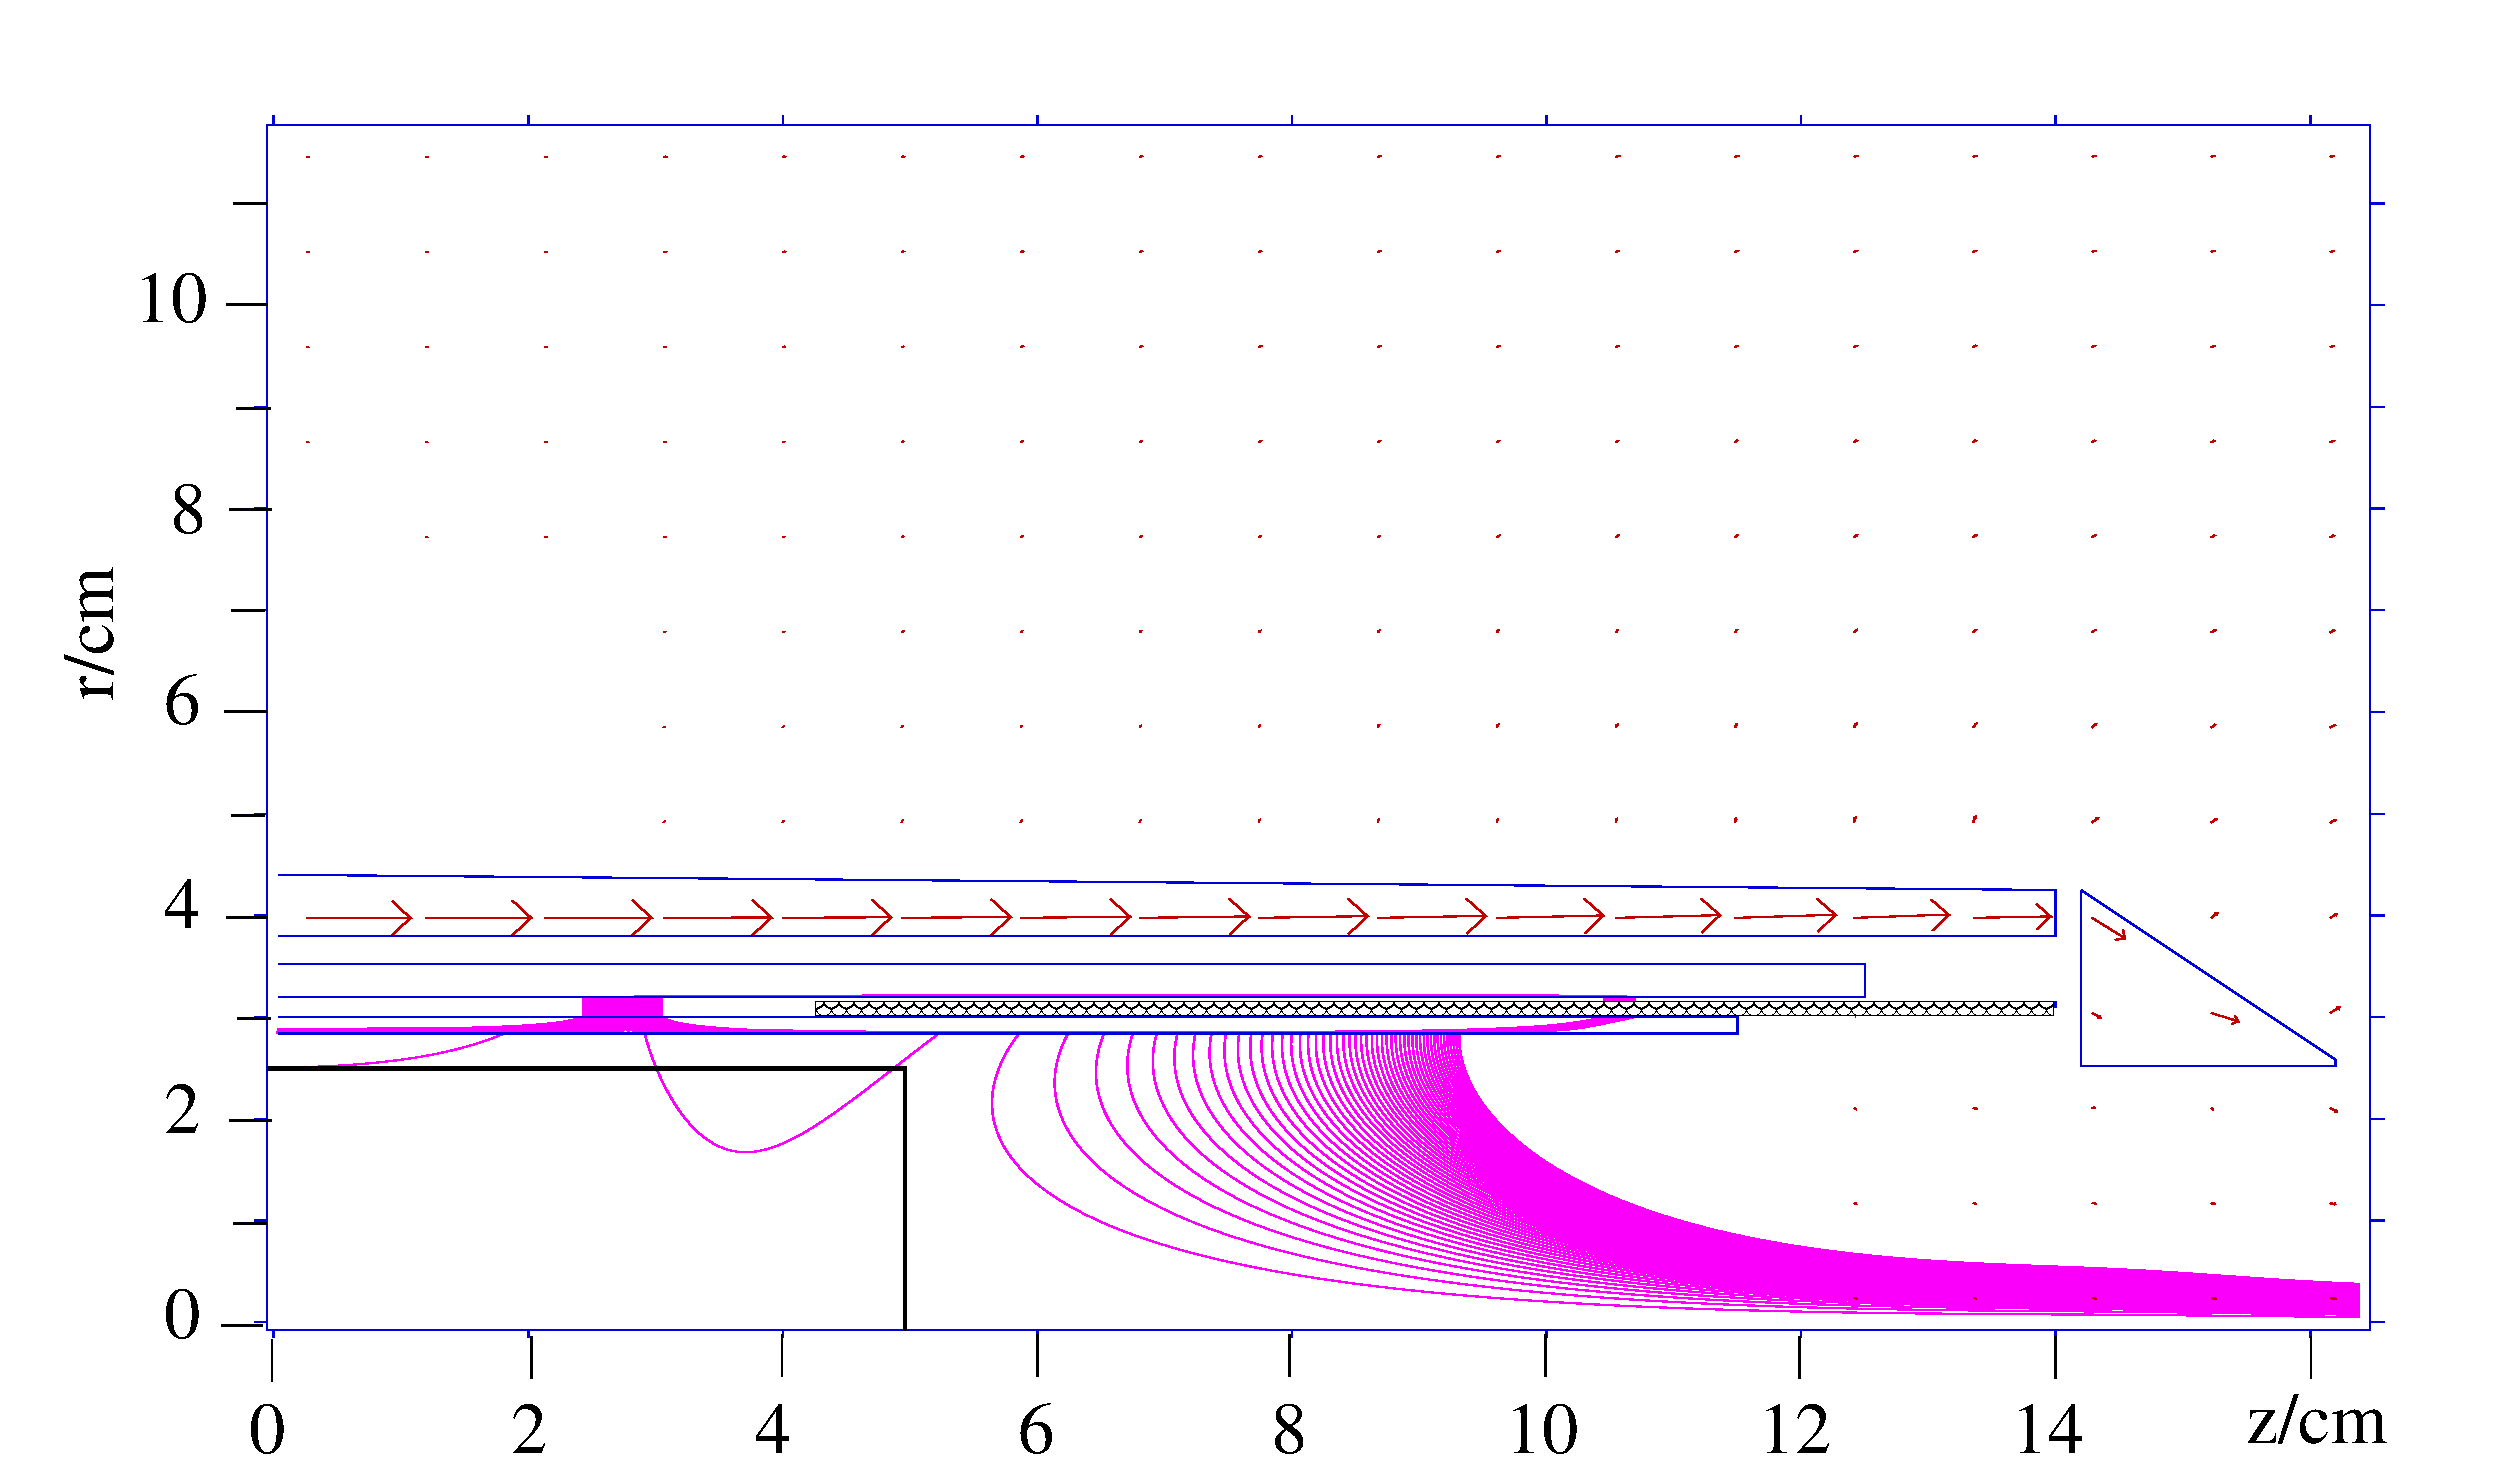
\includegraphics[height=4.75cm]{Tapered400G.eps}\label{VBT3CYUS1}}
\qquad
\subfloat[]
%{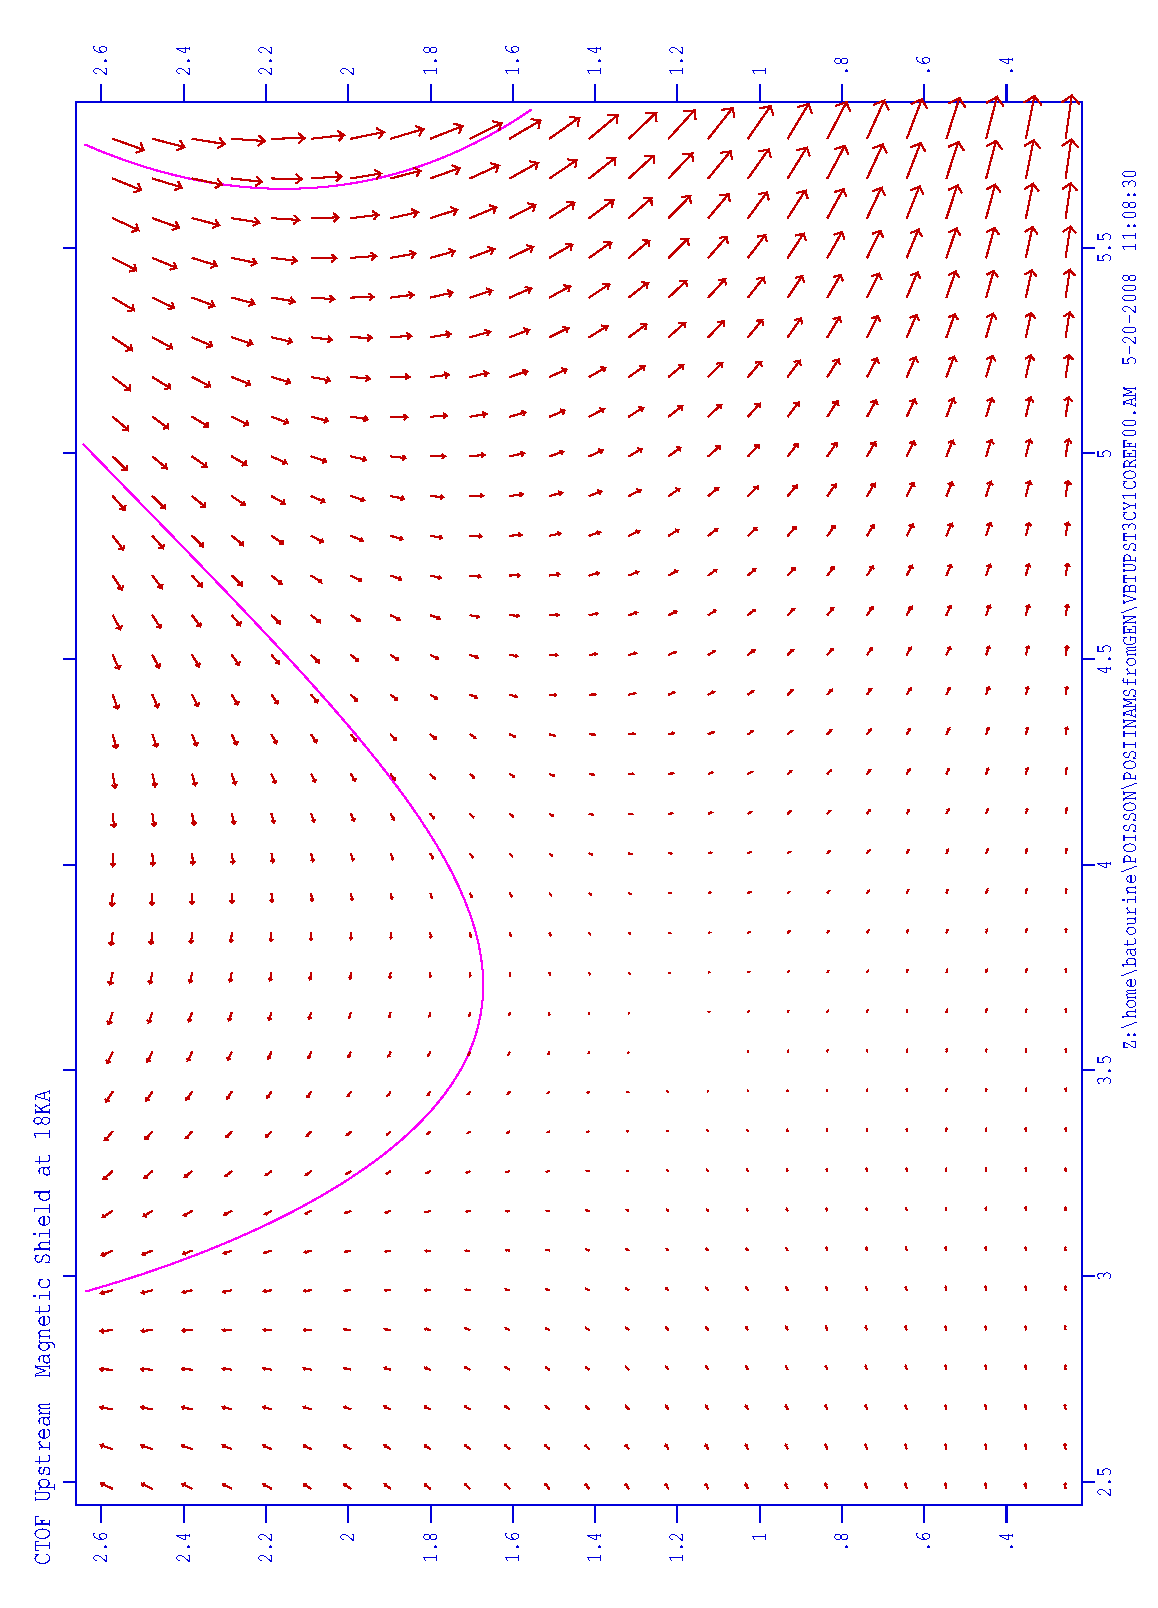
\includegraphics[height=7cm,angle=-90]{VBTUPST3CY1COREF0002.eps}\label{VBT3CYUS2}}
{
\includegraphics[height=4.75cm]{Tapered400Gzoom.eps}\label{VBT3CYUS2}}
\caption{(a). Dynamical magnetic shield in a 400-G axial external field. The
demagnetizing coil indicated by the hatched line. Vertical scale - $r$/cm; horizontal 
scale - $z$/cm. The PMT occupies a box (black line) with $(z,r)$-coordinates (0,0) 
and (5,2.3). (b). Zoomed-in field map in the PMT area. The arrow lengths indicate 
the field magnitudes; the longest arrow is for 1~G.}
\end{figure}
%%%%%%%%%%%%%%%%%%%%%%%%%%%%%%%%%%%%%%%%%%%%%%%%%%%%%%%%%%%%%%%%%%%%%%%%%%%

The shield shown in Fig.~\ref{VBT3CYUS1} may be used for the upstream PMTs of
the CTOF detector where the 1.5-m-long light guides are required to locate the
PMTs in a region of external field of about 400~G. For a 400-G external axial 
field, the total current through all winds of the compensating coil is 
$\approx$100~AW, while the total length of the coil is $\approx$200~mm. Therefore, 
the coil may consist of 200 winds of 1-mm-thick wire with a small current of 0.5~A 
through the wire. That implies a very low power dissipation. This conclusion is of 
high practical importance, since keeping the current below $\approx2$A per mm$^2$ 
prevents the coil from overheating.

We have verified with POISSON calculations that higher fields may be  
exterminated with a thicker outer layer and/or higher currents in the coil.
Thus, this dynamical magnetic shield looks very promising. Therefore, we have 
further developed and prototyped such a shield. In Section~\ref{sec:tests} we 
describe our first real dynamical shield and experimental tests using this shield.

\subsection{Downstream Tapered Dynamical Shield (High Field)}
\label{sec:tapered}

The downstream magnetic shields have to provide shielding against the 1000~G 
external field. Therefore, the external layer has to be thicker than for the
upstream CTOF shields in order to avoid ferromagnetic saturation. In our previous 
calculations shown in Section~\ref{sec:tlfs}, it was observed that the bulk field 
in the outermost shielding layer was non-uniform across the length of the shield, 
becoming greater towards the median plane ($z=0$) of the cylinder. This effect may 
be seen, for example, in Fig.~\ref{R2083_Initial_Iron}, where we notice that the 
field lines that are captured by the outer cylinder are almost normal to its surface. 
Then, due to the very high permeability of the ferromagnetic material, all field 
lines inside the cylinder run almost parallel to the PMT axis. Hence, the magnetic 
flux density increases towards the median plane of the cylinder and reaches its 
maximum at $z$=0, i.e. in the middle of the cylinder. It is precisely at this
location where the effect of ferromagnetic saturation may first occur. In the vicinity 
of the median plane the external field lines are almost normal to the surface (see 
Fig.~\ref{R2083_Initial_Iron}). Therefore, they efficiently penetrate through a 
``gap'' created by a saturated ferromagnetic into the PMT area, which explains the 
shield performance collapse with increasing shield length (the dimensional effect
discussed in Section~\ref{sec:ednmics}). 

In order to make the magnetization more uniform across the outer shielding
cylinder, we have improved the design by using a tapered cylinder, the 
thickness of which linearly increases towards the median plane. The design with 
the tapered outer cylinder, in combination with the demagnetizing coil between 
the two innermost layers, is shown in Fig.~\ref{Tapered_Shield_Design}. The 
outermost shield is composed of soft iron, beginning with a thickness of 1.0~cm 
and slowly increasing to 1.7~cm. Since both the magnetic field flux and the material 
thickness increase linearly towards the middle of the cylinder, the magnetic field 
density in the bulk of ferromagnetic is almost constant. This allows us to maximize 
the magnitude of the permeability, as well as its uniformity along the cylinder.
This design allows us to achieve significantly lower and more uniform fields inside 
the tapered cylinder, which improves the shielding of the inner layers. 

The middle layer is made of 3-mm-thick Hiperm-49, while the inner layer is 
0.8-mm-thick CO-NETIC. Both layers operate in more uniform field compared
to the case of a non-tapered external cylinder. 

The performance of this shield was studied first with POISSON calculations
for an external solenoidal field of 1000~G and varying the current through the 
compensating coil. As in our previous tests, we monitored the field values 
inside the PMT at four reference points. The resulting fields as a function of 
the coil current are shown in Fig.~\ref{Tapered_Shield_0.3cm_PMT_Region}. It is 
observed that the internal magnetic field in the PMT region is at the level of 
0.1~G at a coil current of 20-30~AW. It is also of interest to note that at this 
high external magnetic field, none of three ferromagnetic cylinders has reached 
saturation. Thus, the dynamical shield is an excellent candidate for the PMT shield 
in the CTOF detector.

%%%%%%%%%%%%%%%%%%%%%%%%%%%%%%%%%%%%%%%%%%%%%%%%%%%%%%%%%%%%%%%%%%%%%%%%%%%%%%%%%%
\begin{figure}[htbp]
\centering
\subfloat[]
{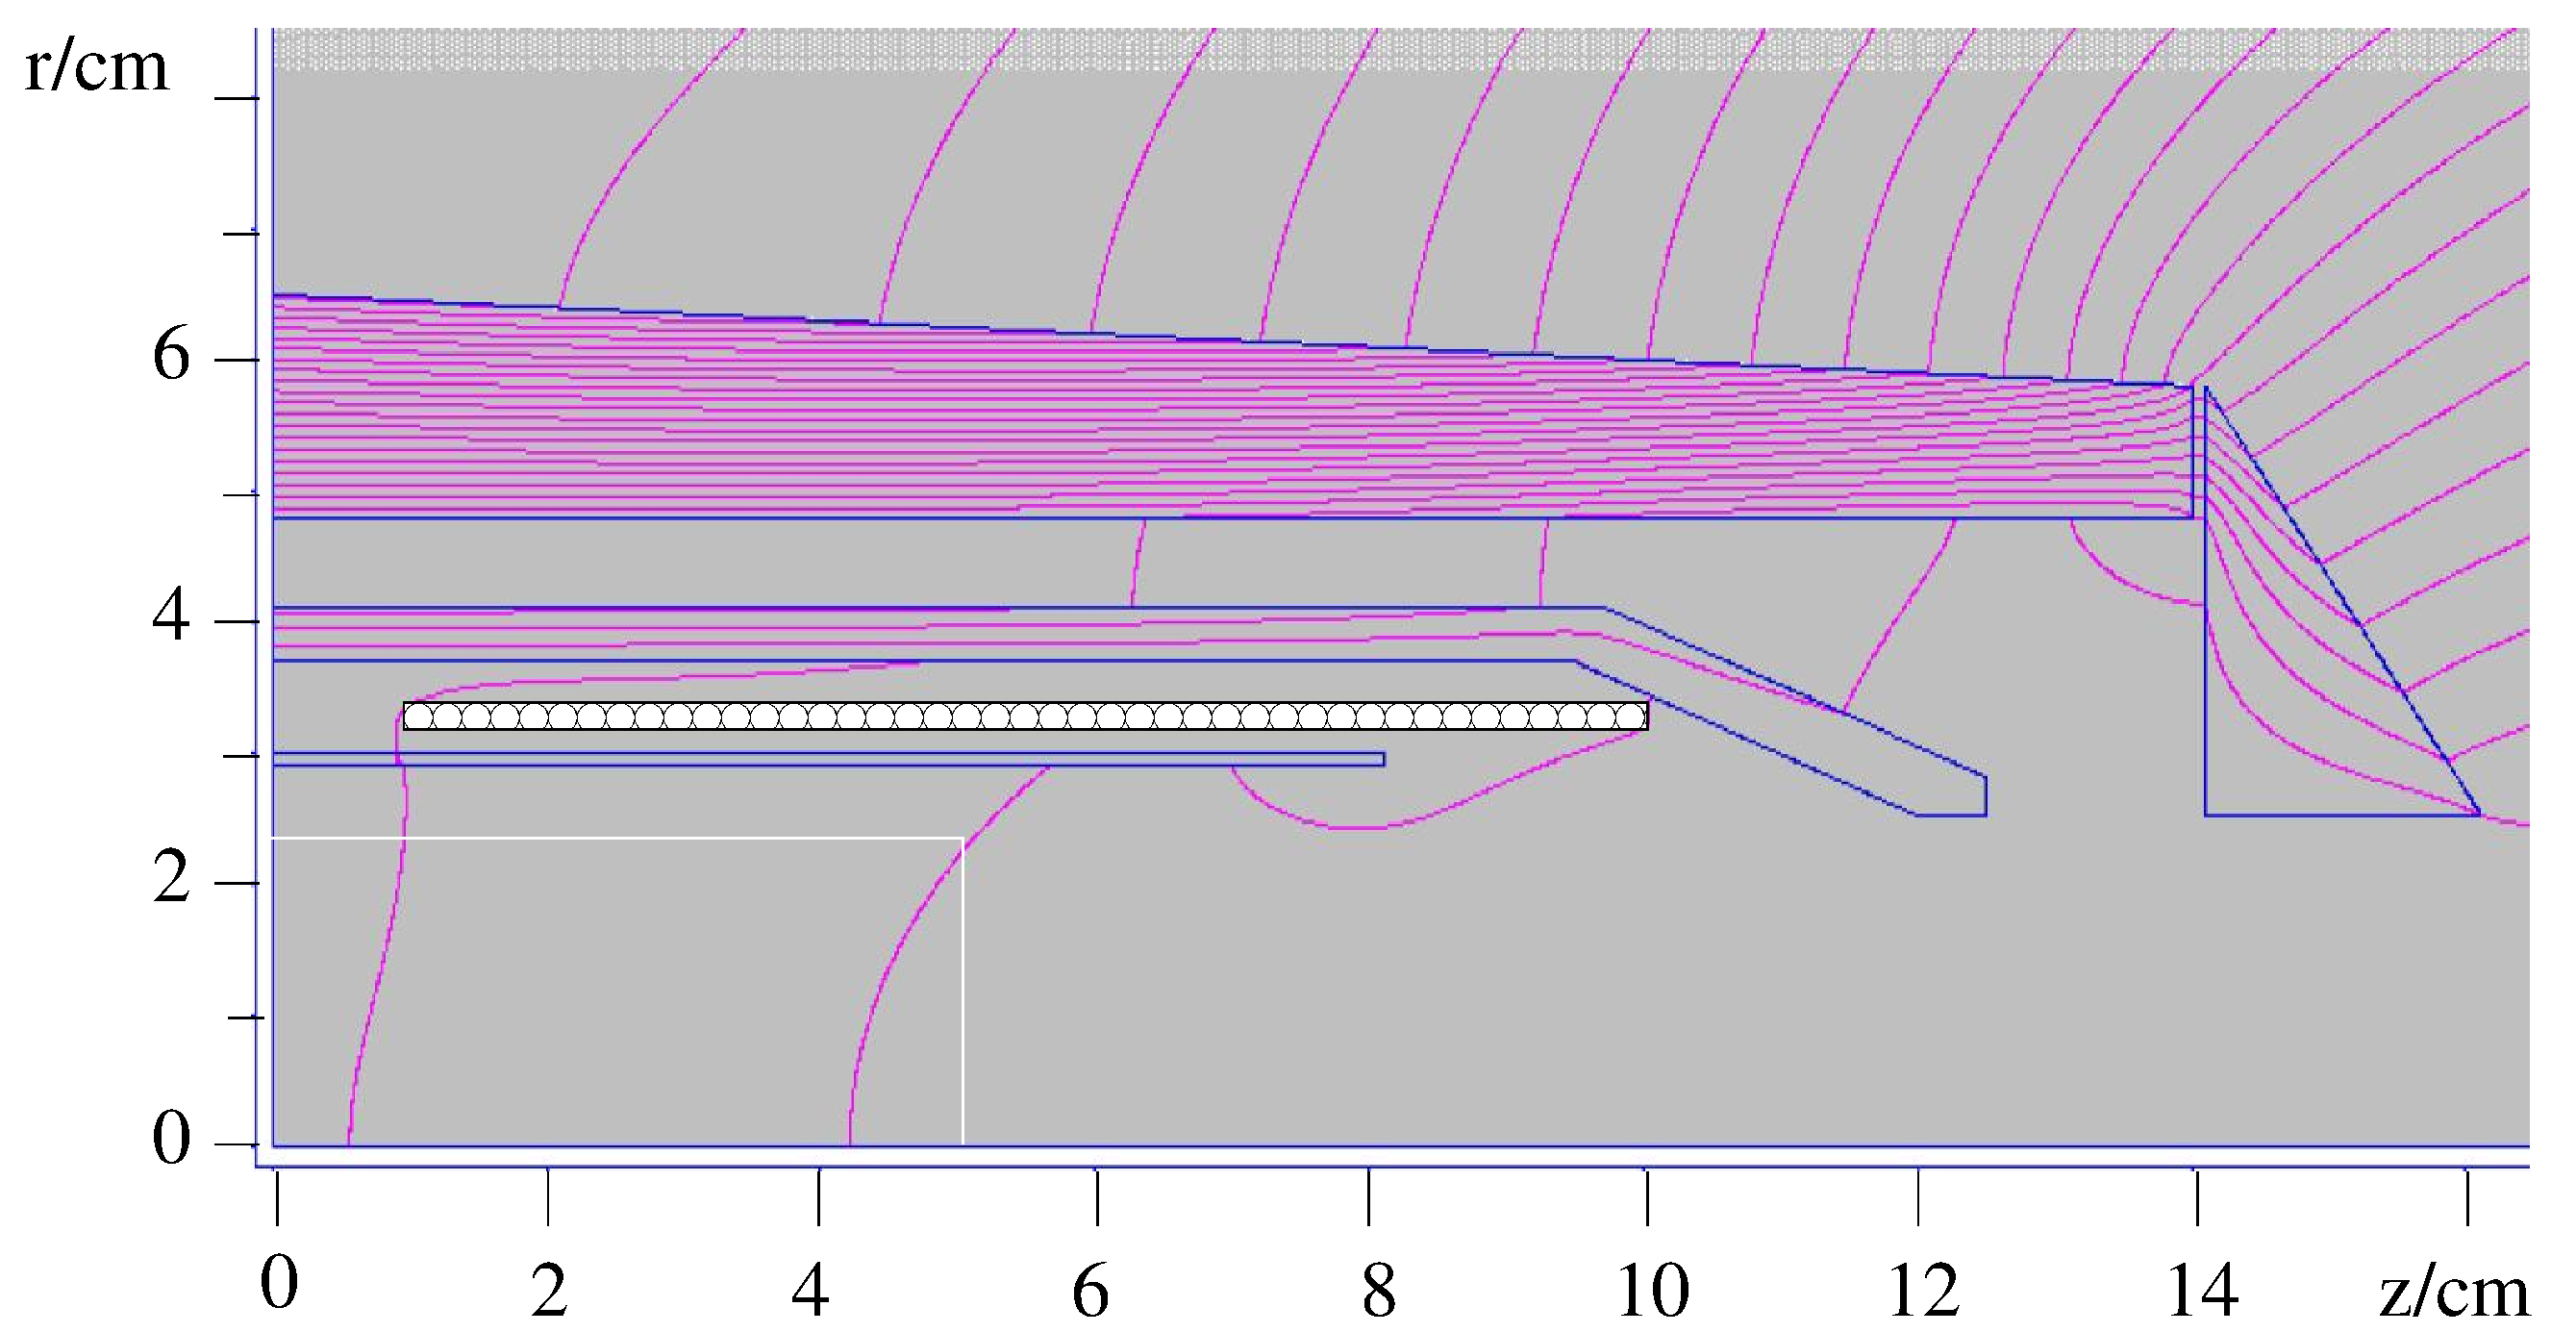
\includegraphics[height=4.5cm,clip=true,bb=0 0 1300 700]{R2083_Iron_hiperm49_CONETIC_TaperedShieldDesign.eps}
%{\includegraphics[height=4.5cm,clip=true,bb=0 0 1300 700]{Tapered.eps}
\label{Tapered_Shield_Design}}
\qquad
\subfloat[]	
{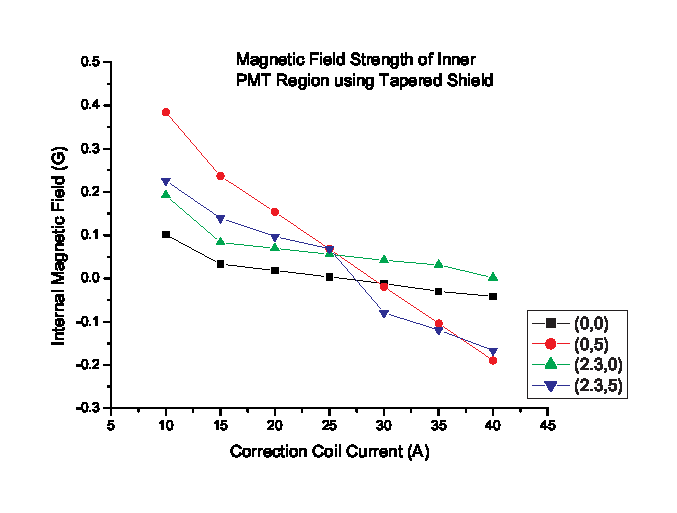
\includegraphics[height=4.cm,clip=true,bb= 10 15 300 190]{R2083_Tapered_0.3cmMiddle_PMT_Region.eps}
\label{Tapered_Shield_0.3cm_PMT_Region}}
\caption{(a). POISSON model of a tapered dynamical magnetic shield in an
external 1000~G axial field. Horizontal scale $z$/cm; vertical scale -$r$/cm. 
The outermost tapered cylinder is 10-mm to 17-mm-thick iron. The middle cylinder 
is 3-mm-thick Hiperm-49. The inner cylinder is 0.8-mm-thick CO-NETIC. The 
correction coil (thick white line at $r$=3.3~cm) current is set to 25~AW. 
(b). The magnetic field at our four reference points in the PMT region (white box
in the lower-left corner of (a)) as a function of the coil current shown in $AW$ 
(horizontal scale). The coordinates of the reference points are labeled as $(r,z)$.}
\label{Tapered_Shield_0.3cm}
\end{figure}
%%%%%%%%%%%%%%%%%%%%%%%%%%%%%%%%%%%%%%%%%%%%%%%%%%%%%%%%%%%%%%%%%%%%%%%%%%%%%%%%%%

\subsection{Prototyping and Effectiveness Measurements}
\label{sec:tests}

In this section we describe our prototype studies of the dynamical magnetic shield. 
Its tapered design is shown in Fig.~\ref{fig:DMS} and it is very close to the 
tapered model described in Section~\ref{sec:tapered}. A photograph of the dynamical 
shield components is shown in Fig.~\ref{DMSPHOTO}. The outermost 28-cm-long shield 
layer was fabricated from 1018 steel. The innermost ferromagnetic was made of 
0.8-mm-thick mu-metal, which is a slightly worse ferromagnetic than CO-NETIC. The 
middle layer material was 3.2-mm-thick Hiperm-49. The demagnetizing coil has 
100 winds of 1-mm-thick copper wire.

%%%%%%%%%%%%%%%%%%%%%%%%%%%%%%%%%%%%%%%%%%%%%%%%%%%%%%%%%%%%%%%%%%%%%%%%%%%%%%%%%
\begin{figure}[htbp]
\includegraphics[width=12cm,clip=true,bb= -30 050 550 350]{DMS-1.ps.gz}
\caption{Dynamical magnetic shield: 1 - external layer of iron, 2 - middle layer 
of Hiperm-49, 3 - innermost layer of CO-NETIC, 4 - solenoid wind around the 
innermost layer of ferromagnetic, 5 - shield cone, 6 - shield cone, 7 - shielded 
area with low field, 8 - direct current power supply. Units on all dimensions
shown are in mm.}
\label{fig:DMS}
\end{figure}
%%%%%%%%%%%%%%%%%%%%%%%%%%%%%%%%%%%%%%%%%%%%%%%%%%%%%%%%%%%%%%%%%%%%%%%%%%%%%%%%%

The shielding properties of this dynamic magnetic shield were measured using a 
superconducting 5-T solenoid to generate the external magnetic field. The prototype 
was placed in the center of the solenoid bore (130~mm in diameter). The magnetic 
field profile along the bore axis is shown in Fig.~\ref{SOLFIELD}. As seen from 
this figure, within the space occupied by the prototype, the solenoid inner field 
is almost uniform in magnitude.

%%%%%%%%%%%%%%%%%%%%%%%%%%%%%%%%%%%%%%%%%%%%%%%%%%%%%%%%%%%%%%%%%%%%%%%%%%%%%%%%%
\begin{figure}[htbp]
\centering
\subfloat[]
%{\includegraphics[height=4cm,clip=true,bb=10 -50 1350 750 ]{dynamicalshield.eps}
{\includegraphics[height=4cm,clip=true,bb=100 300 3800 2600]{dynamicalshield1.eps}
\label{DMSPHOTO}}
\qquad
\subfloat[]	
{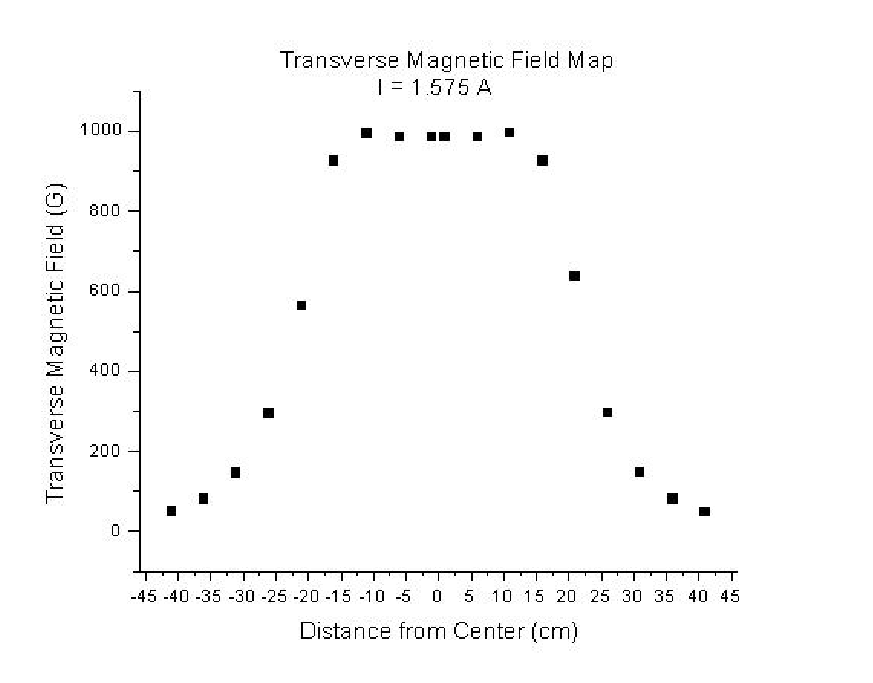
\includegraphics[height=4cm,clip=true,bb= 10 10 350 270]{solfieldprofile.eps}
\label{SOLFIELD}}
\caption{(a). Tapered dynamical magnetic shield. The outermost tapered cylinder is 
10-mm to 17-mm-thick iron. The middle cylinder is 3-mm-thick Hiperm-49. The inner 
cylinder is 0.8-mm-thick CO-NETIC wrapped by the wire of the correction coil. 
(b). The magnitude of the external field created by the solenoid as a function of 
the coordinate along the solenoid axis. The region of constant field magnitude is 
about 30-cm wide.}
\label{Tapered_Shield_photh}
\end{figure}
%%%%%%%%%%%%%%%%%%%%%%%%%%%%%%%%%%%%%%%%%%%%%%%%%%%%%%%%%%%%%%%%%%%%%%%%%%%%%%%%%

Axial and radial Hall probes from a gaussmeter were stepped along and across 
the PMT space with a 1-cm increment. The performance of the dynamical shield was 
tested up to a maximum tolerated field of 910~G. The measured inner field 
profiles at the maximum tolerated field are shown in Fig.~\ref{innergauss}.
Here it is seen that at a demagnetizing current of 1.5~A, both the axial and
radial magnetic field components (see Fig.~\ref{axiprob} and Fig.~\ref{radprob},
respectively) are within the tolerable level below 0.2~G. Considering that 
the permeability of the ferromagnetic samples may differ from their material 
specifications, the measured field magnitudes and demagnetizing currents may be 
considered to be in good accordance with the POISSON calculations from 
Section~\ref{sec:tapered}.

%%%%%%%%%%%%%%%%%%%%%%%%%%%%%%%%%%%%%%%%%%%%%%%%%%%%%%%%%%%%%%%%%%%%%%%%%%%%%%%%%
\begin{figure}[htbp]
\centering
\subfloat[]
{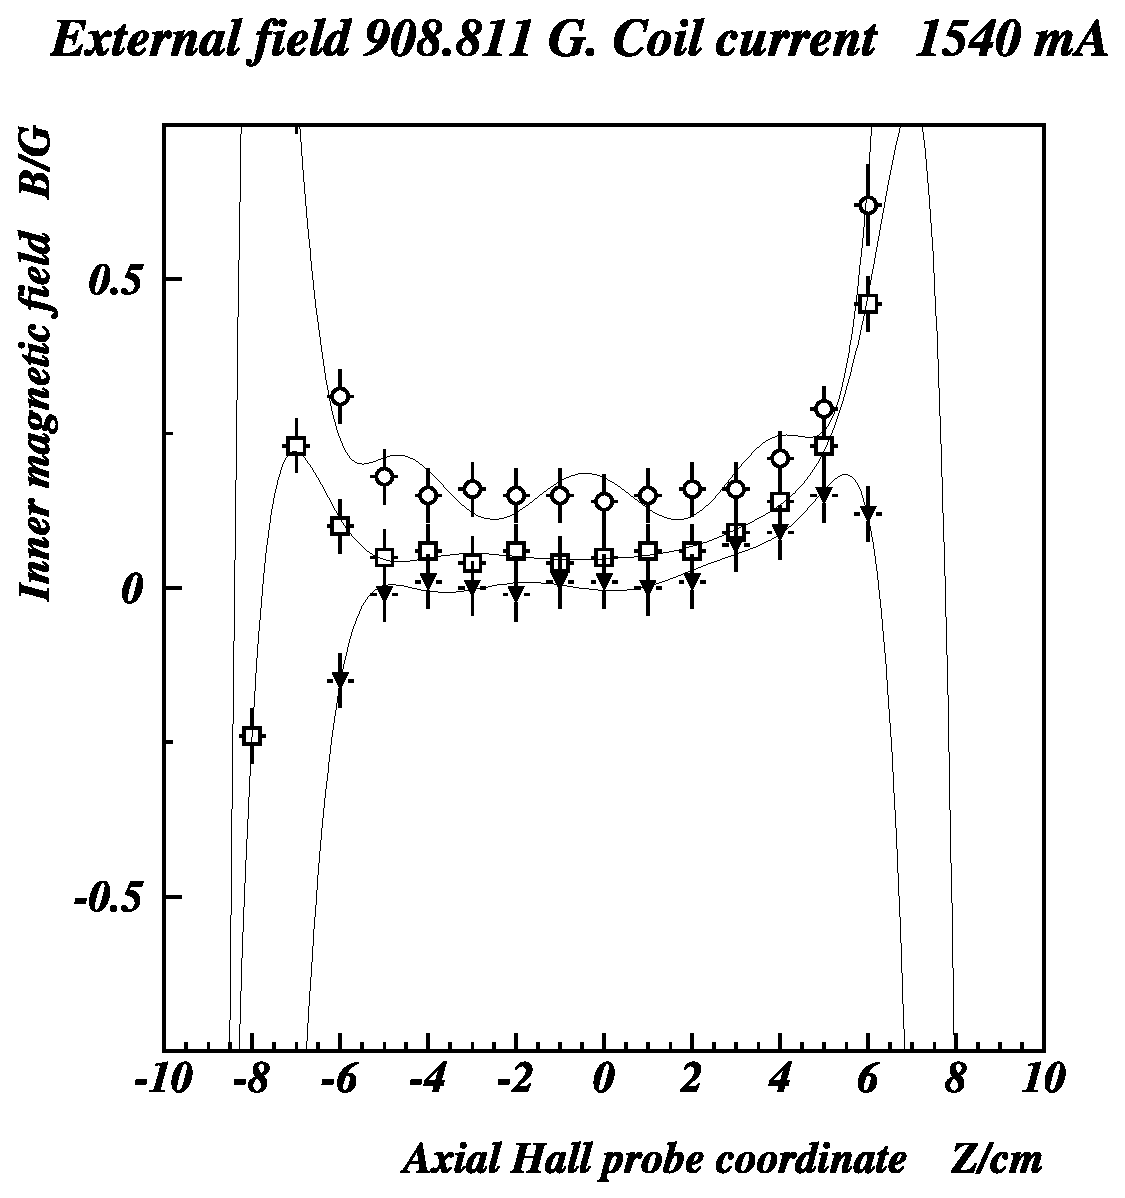
\includegraphics[height=6cm,clip=true,bb=30 150 580 680]{shield908axialprobe.eps}
\label{axiprob}}
\qquad
\subfloat[]
{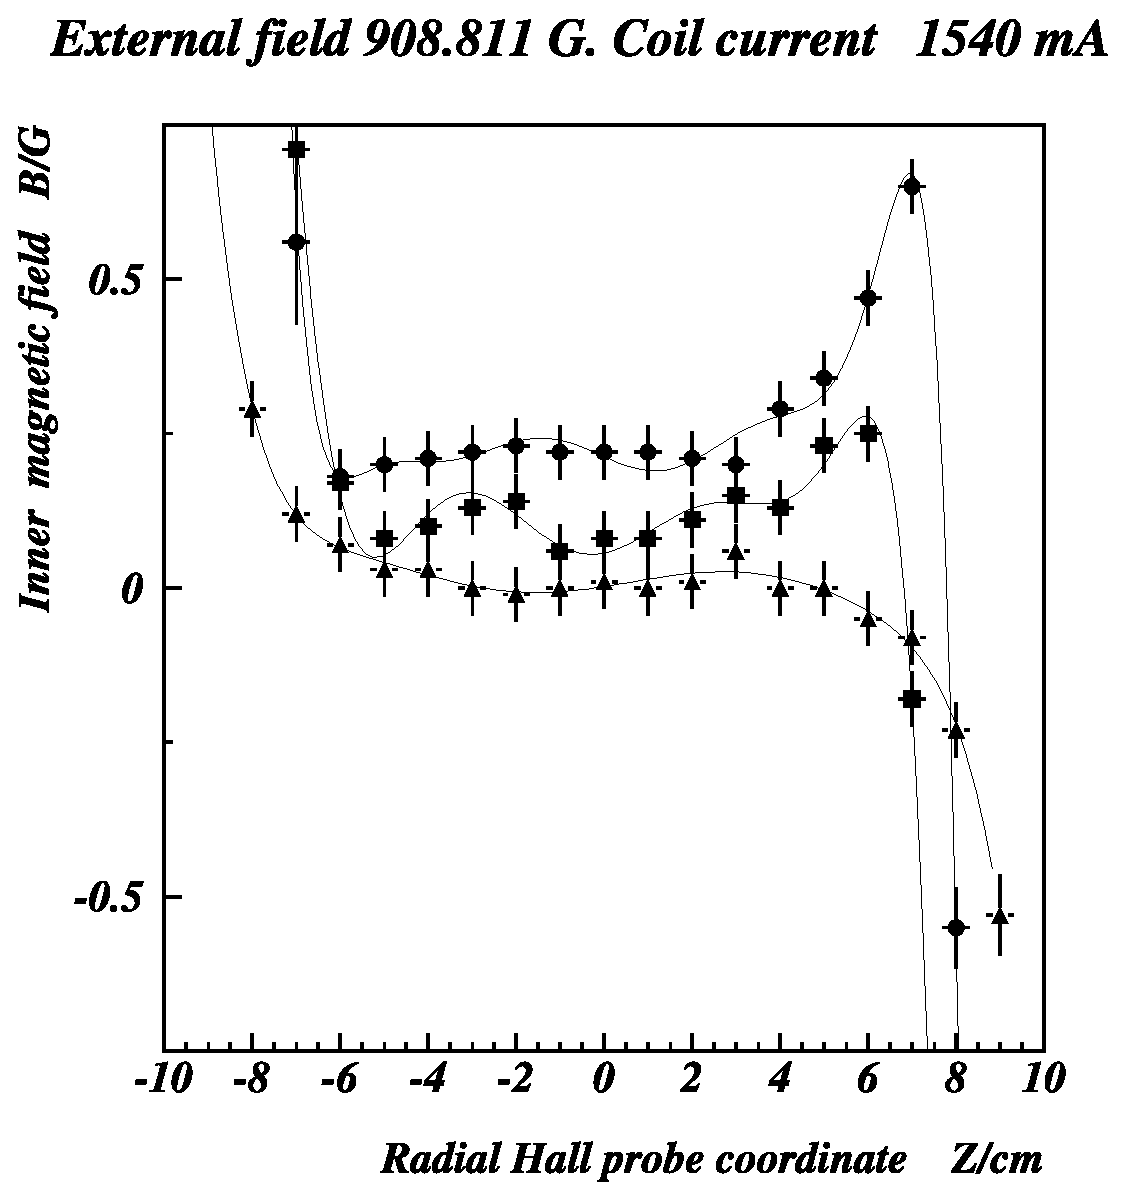
\includegraphics[height=6cm,clip=true,bb=30 150 560 680]{shield908radialprobe.eps}
\label{radprob}}
\caption{Measured inner field of the dynamical magnetic shield in a 910-G external 
solenoidal field. (a). Axial and (b). radial components of the inner field at a 
coil current 1.54~A. The curves are only to guide the eye.}
\label{innergauss}
\end{figure}
%%%%%%%%%%%%%%%%%%%%%%%%%%%%%%%%%%%%%%%%%%%%%%%%%%%%%%%%%%%%%%%%%%%%%%%%%%%%%%%%%%

Tolerable fields below 0.2~G were achieved in a cylindrical area of size
$4 \times 10$~cm$^2$.  This volume is sufficient to house the accelerating system 
of our nominal Hamamatsu R2083 PMT for the CTOF detector readout. Hence, the 
dynamical magnetic shield demonstrates excellent performance with a shielding factor 
$S$=5000 in external axial fields up to 910~G. Further increase of the external
field beyond 910~G results in a rapid climbing of the inner fields due to saturation 
effects in the ferromagnetic materials.

\section{Conclusions}
\label{sec:concl}

We have developed a simple theory of a ferromagnetic shield in an axial magnetic 
field  that   allows for a clear and unambiguous interpretation of numerical net 
calculations via the POISSON program. Such calculations were performed for various 
multi-layer shield configurations for both the upstream and downstream regions of 
the CTOF detector. These calculations have demonstrated that the dynamics of coaxial 
ferromagnetic cylinders is very complex and, sometimes, surprising. Some unexpected 
effects were manifested by the models, such as performance collapse with increasing 
shield length. This effect was predicted by our simple theory.

With the help of the POISSON program, we have designed a single-layer ferromagnetic 
shield that may sufficiently protect metal-channel PMTs up to axial fields of 
2500~G. However, given the restrictions from the design with Hamamatsu R2083 
linear-focused PMTs, a shielding solution with a multi-layer passive ferromagnetic 
shield was not possible. However, even such an advanced shield will only be effective 
to satisfy a 0.5-G inner field tolerance. In order to obtain fields below 0.2~G 
inside the accelerating system of the PMTs, we have developed a novel dynamical 
magnetic shield that consists of ferromagnetic layers and a solenoid between the 
layers. Such a shield was tested both within our POISSON models and with an 
experimental prototype. The dynamical shield has demonstrated excellent performance 
that meets our 0.2~G specification in the PMT volume in external axial magnetic 
fields up to 910~G. Additionally, a more uniform field inside the PMT has been 
achieved using a tapered design for the external ferromagnetic cylinder. 

\paragraph{Acknowledgments.}
We appreciate the assistance of Dr. Eugene Chudakov for helping to set up
the POISSON model and for other valuable advice. We also express our gratitude 
to Dr. Chris Keith, Chris Carlin, and James Brock for the technical 
support during the shield tests.

\begin{thebibliography}{99}

\bibitem{clas12} 
Jefferson Laboratory Hall B CLAS12 Technical Design Report 2009.\\
http://www.jlab.org/Hall-B/clas12\_tdr.pdf

\bibitem{r1} 
V.N. Batourine {\it et al.}, %``Measurements of PMT Time Resolution at Kyungpook National University'', 
CLAS-Note 2004-16, (2004).\\
http://www1.jlab.org/ul/Physics/Hall-B/clas/public/2004-016.pdf

\bibitem{cn200439} 
V.N. Batourine {\it et al.}, %``Studies of Time Resolution of the Burle 85001 Micro-channel Plate Photomultipliers in Comparison with Standard PMTs'',
CLAS-Note 2004-39, (2004).\\
http://www1.jlab.org/ul/Physics/Hall-B/clas/public/2004-039.pdf

\bibitem{llg}  
V. Batourine {\it et al.}, % ``Status Report on the Studies at Kyungpook National University in 2005'',
CLAS-Note 2005-003, (2005).\\
http://www1.jlab.org/ul/Physics/Hall-B/clas/public/2005-003.pdf

\bibitem{cn85011}  
F. Barbosa {\it et al.}, % ``Status and Further Steps Towards the CLAS12 
%Start Counter'', 
CLAS-Note 2006-011, (2006).\\
http://www1.jlab.org/ul/Physics/Hall-B/clas/public/2006-011.pdf

\bibitem{Baturin:2005} 
V. Baturin {\it et al.}, % ``Time-of-Flight Resolution of Scintillating Counters with Burle 85001 Micro-channel Plate Photomultipliers in Comparison with Hamamatsu R2083'', 
Nucl. Instr. and Meth. A {\bf 562}, 327 (2006).

\bibitem{6percent} 
V. Baturin {\it et al.}, % ``Time Resolution Measurements with the Final Prototype for the CLAS12 Central TOF Detector.'', 
CLAS-Note 2009-001, (2009).\\
http://www1.jlab.org/ul/Physics/Hall-B/clas/public/2009-001.pdf


\bibitem{poisson}
K. Halbach and R.F. Holsinger, Part. Acc. {\bf 7}, 213 (1976).

\bibitem{r2} 
E.S. Smith {\it et al.}, % ``The Time-of-Flight System for CLAS'',  
Nucl. Instr. and Meth. A {\bf 432}, 265 (1999).


\bibitem{flint} 
J. Flint and E. Smith, % ``Tests of Phillips XP4312/D1 PMTs in a Magnetic Field''
CLAS-Note 94-008,(1994).\\
http://www.jlab.org/Hall-B/notes/clas\_notes94/note94-008.pdf

\bibitem{eltongluex}
E.S.Smith, GlueX-doc-843.\\
http://argus.phys.uregina.ca/gluex/DocDB/0008/000843/002/bshield.pdf

\bibitem{grilli}
Calculations by D. Grilli, Mu-Shield Company, private communication.

\bibitem{dynshi} 
V. Baturin {\it et al.}, % ``Dynamic Magnetic Shields for the CLAS12 Central TOF Detector'', 
CLAS-NOTE~2008-034, (2009)\\
http://www1.jlab.org/ul/Physics/Hall-B/clas/public/2008-034.pdf

\bibitem{wieland}
B.M. Wieland, ``Advanced Studies of the Photomultiplier Tube Magnetic 
Shielding for the CLAS12 Central Time of Flight Counter", Senior Thesis,
Old Dominion University, 2009.

\bibitem{jackson}
J.D. Jackson, ``Classical Electrodynamics'', John Wiley \& Sons, 3rd ed., New York, 1998. 

\end{thebibliography}

\end{document}
